% Created by tikzDevice version 0.12.6 on 2024-05-22 16:04:32
% !TEX encoding = UTF-8 Unicode
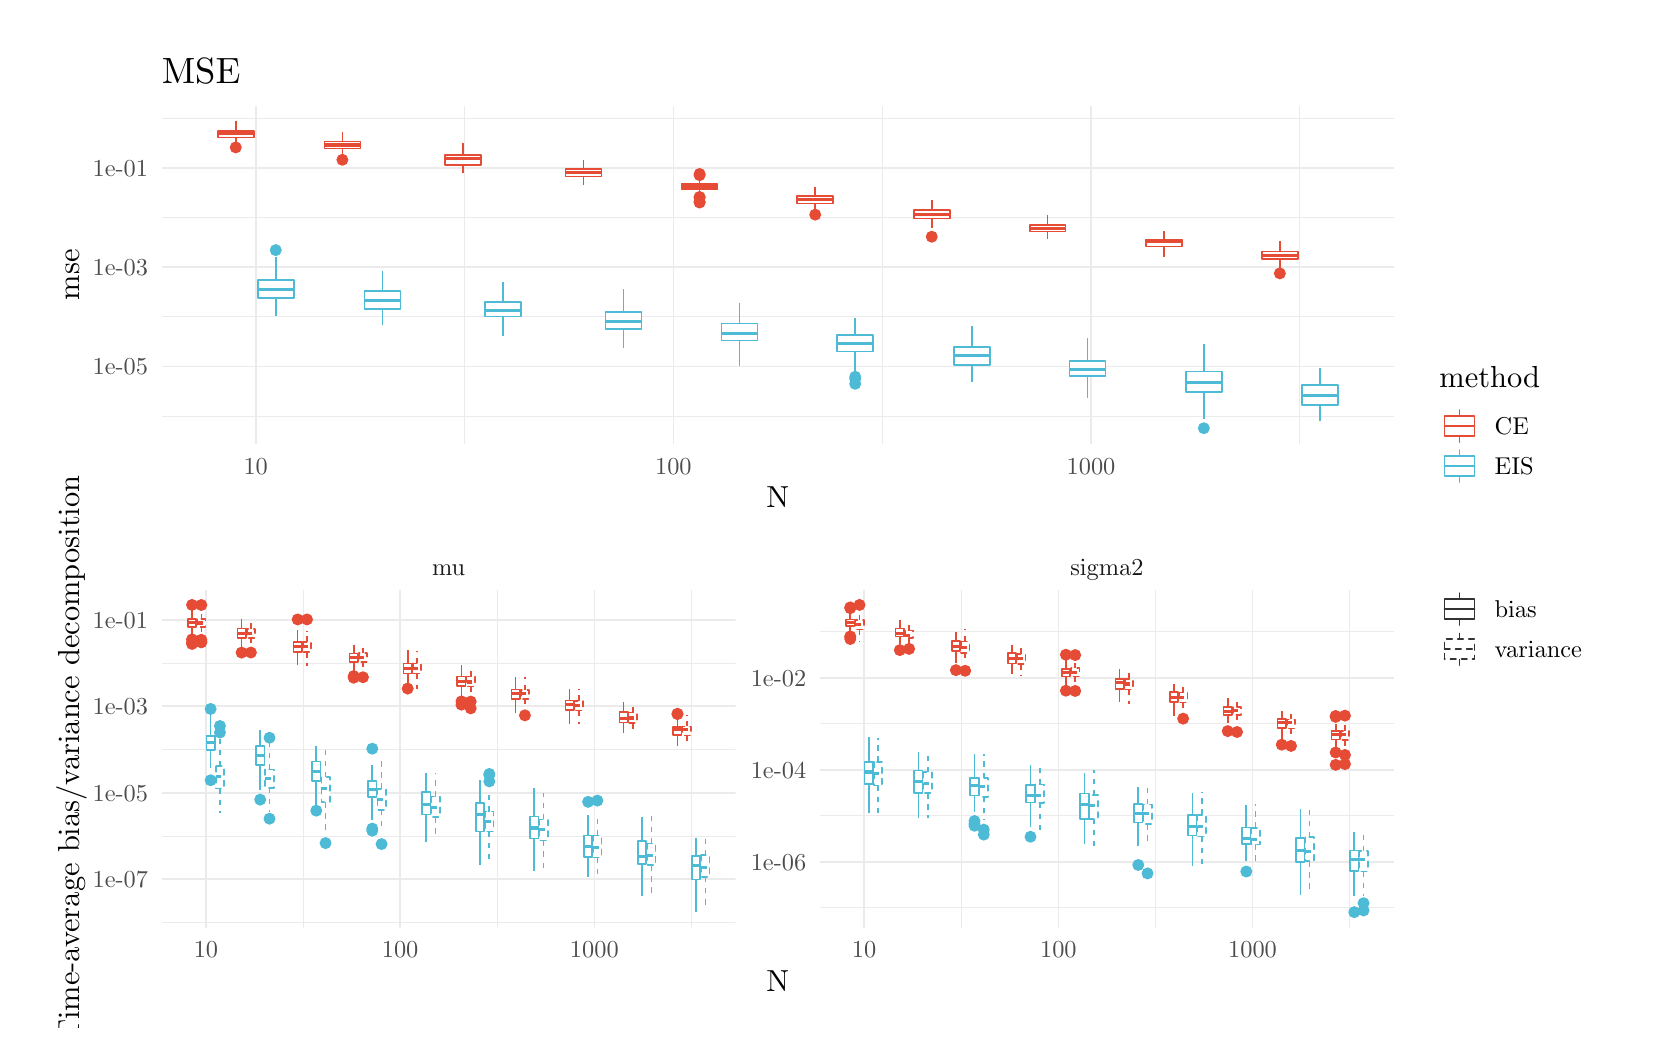
\begin{tikzpicture}[x=1pt,y=1pt]
\definecolor{fillColor}{RGB}{255,255,255}
\path[use as bounding box,fill=fillColor,fill opacity=0.00] (0,0) rectangle (578.16,361.35);
\begin{scope}
\path[clip] ( 48.45,211.07) rectangle (493.66,333.19);
\definecolor{drawColor}{gray}{0.92}

\path[draw=drawColor,line width= 0.3pt,line join=round] ( 48.45,220.95) --
	(493.66,220.95);

\path[draw=drawColor,line width= 0.3pt,line join=round] ( 48.45,256.83) --
	(493.66,256.83);

\path[draw=drawColor,line width= 0.3pt,line join=round] ( 48.45,292.70) --
	(493.66,292.70);

\path[draw=drawColor,line width= 0.3pt,line join=round] ( 48.45,328.58) --
	(493.66,328.58);

\path[draw=drawColor,line width= 0.3pt,line join=round] (157.87,211.07) --
	(157.87,333.19);

\path[draw=drawColor,line width= 0.3pt,line join=round] (308.79,211.07) --
	(308.79,333.19);

\path[draw=drawColor,line width= 0.3pt,line join=round] (459.70,211.07) --
	(459.70,333.19);

\path[draw=drawColor,line width= 0.6pt,line join=round] ( 48.45,238.89) --
	(493.66,238.89);

\path[draw=drawColor,line width= 0.6pt,line join=round] ( 48.45,274.76) --
	(493.66,274.76);

\path[draw=drawColor,line width= 0.6pt,line join=round] ( 48.45,310.64) --
	(493.66,310.64);

\path[draw=drawColor,line width= 0.6pt,line join=round] ( 82.41,211.07) --
	( 82.41,333.19);

\path[draw=drawColor,line width= 0.6pt,line join=round] (233.33,211.07) --
	(233.33,333.19);

\path[draw=drawColor,line width= 0.6pt,line join=round] (384.24,211.07) --
	(384.24,333.19);
\definecolor{drawColor}{RGB}{230,75,53}
\definecolor{fillColor}{RGB}{230,75,53}

\path[draw=drawColor,line width= 0.4pt,line join=round,line cap=round,fill=fillColor] ( 75.19,318.08) circle (  1.96);

\path[draw=drawColor,line width= 0.6pt,line join=round] ( 75.19,324.10) -- ( 75.19,327.64);

\path[draw=drawColor,line width= 0.6pt,line join=round] ( 75.19,321.70) -- ( 75.19,318.11);
\definecolor{fillColor}{RGB}{255,255,255}

\path[draw=drawColor,line width= 0.6pt,line join=round,line cap=round,fill=fillColor] ( 68.69,324.10) --
	( 68.69,321.70) --
	( 81.69,321.70) --
	( 81.69,324.10) --
	( 68.69,324.10) --
	cycle;

\path[draw=drawColor,line width= 1.1pt,line join=round] ( 68.69,322.94) -- ( 81.69,322.94);
\definecolor{fillColor}{RGB}{230,75,53}

\path[draw=drawColor,line width= 0.4pt,line join=round,line cap=round,fill=fillColor] (113.72,313.60) circle (  1.96);

\path[draw=drawColor,line width= 0.6pt,line join=round] (113.72,320.25) -- (113.72,323.73);

\path[draw=drawColor,line width= 0.6pt,line join=round] (113.72,317.63) -- (113.72,314.35);
\definecolor{fillColor}{RGB}{255,255,255}

\path[draw=drawColor,line width= 0.6pt,line join=round,line cap=round,fill=fillColor] (107.21,320.25) --
	(107.21,317.63) --
	(120.22,317.63) --
	(120.22,320.25) --
	(107.21,320.25) --
	cycle;

\path[draw=drawColor,line width= 1.1pt,line join=round] (107.21,318.95) -- (120.22,318.95);

\path[draw=drawColor,line width= 0.6pt,line join=round] (157.30,315.23) -- (157.30,319.69);

\path[draw=drawColor,line width= 0.6pt,line join=round] (157.30,311.78) -- (157.30,308.73);

\path[draw=drawColor,line width= 0.6pt,line join=round,line cap=round,fill=fillColor] (150.80,315.23) --
	(150.80,311.78) --
	(163.80,311.78) --
	(163.80,315.23) --
	(150.80,315.23) --
	cycle;

\path[draw=drawColor,line width= 1.1pt,line join=round] (150.80,314.12) -- (163.80,314.12);

\path[draw=drawColor,line width= 0.6pt,line join=round] (200.83,310.36) -- (200.83,313.61);

\path[draw=drawColor,line width= 0.6pt,line join=round] (200.83,307.54) -- (200.83,304.56);

\path[draw=drawColor,line width= 0.6pt,line join=round,line cap=round,fill=fillColor] (194.33,310.36) --
	(194.33,307.54) --
	(207.33,307.54) --
	(207.33,310.36) --
	(194.33,310.36) --
	cycle;

\path[draw=drawColor,line width= 1.1pt,line join=round] (194.33,308.84) -- (207.33,308.84);
\definecolor{fillColor}{RGB}{230,75,53}

\path[draw=drawColor,line width= 0.4pt,line join=round,line cap=round,fill=fillColor] (242.80,299.92) circle (  1.96);

\path[draw=drawColor,line width= 0.4pt,line join=round,line cap=round,fill=fillColor] (242.80,308.48) circle (  1.96);

\path[draw=drawColor,line width= 0.4pt,line join=round,line cap=round,fill=fillColor] (242.80,308.05) circle (  1.96);

\path[draw=drawColor,line width= 0.4pt,line join=round,line cap=round,fill=fillColor] (242.80,300.16) circle (  1.96);

\path[draw=drawColor,line width= 0.4pt,line join=round,line cap=round,fill=fillColor] (242.80,298.43) circle (  1.96);

\path[draw=drawColor,line width= 0.4pt,line join=round,line cap=round,fill=fillColor] (242.80,298.15) circle (  1.96);

\path[draw=drawColor,line width= 0.6pt,line join=round] (242.80,304.97) -- (242.80,307.73);

\path[draw=drawColor,line width= 0.6pt,line join=round] (242.80,303.06) -- (242.80,300.58);
\definecolor{fillColor}{RGB}{255,255,255}

\path[draw=drawColor,line width= 0.6pt,line join=round,line cap=round,fill=fillColor] (236.29,304.97) --
	(236.29,303.06) --
	(249.30,303.06) --
	(249.30,304.97) --
	(236.29,304.97) --
	cycle;

\path[draw=drawColor,line width= 1.1pt,line join=round] (236.29,303.95) -- (249.30,303.95);
\definecolor{fillColor}{RGB}{230,75,53}

\path[draw=drawColor,line width= 0.4pt,line join=round,line cap=round,fill=fillColor] (284.57,293.78) circle (  1.96);

\path[draw=drawColor,line width= 0.6pt,line join=round] (284.57,300.46) -- (284.57,303.76);

\path[draw=drawColor,line width= 0.6pt,line join=round] (284.57,297.82) -- (284.57,294.32);
\definecolor{fillColor}{RGB}{255,255,255}

\path[draw=drawColor,line width= 0.6pt,line join=round,line cap=round,fill=fillColor] (278.07,300.46) --
	(278.07,297.82) --
	(291.07,297.82) --
	(291.07,300.46) --
	(278.07,300.46) --
	cycle;

\path[draw=drawColor,line width= 1.1pt,line join=round] (278.07,299.23) -- (291.07,299.23);
\definecolor{fillColor}{RGB}{230,75,53}

\path[draw=drawColor,line width= 0.4pt,line join=round,line cap=round,fill=fillColor] (326.69,285.81) circle (  1.96);

\path[draw=drawColor,line width= 0.6pt,line join=round] (326.69,295.41) -- (326.69,299.25);

\path[draw=drawColor,line width= 0.6pt,line join=round] (326.69,292.41) -- (326.69,289.08);
\definecolor{fillColor}{RGB}{255,255,255}

\path[draw=drawColor,line width= 0.6pt,line join=round,line cap=round,fill=fillColor] (320.19,295.41) --
	(320.19,292.41) --
	(333.19,292.41) --
	(333.19,295.41) --
	(320.19,295.41) --
	cycle;

\path[draw=drawColor,line width= 1.1pt,line join=round] (320.19,293.87) -- (333.19,293.87);

\path[draw=drawColor,line width= 0.6pt,line join=round] (368.57,290.05) -- (368.57,293.57);

\path[draw=drawColor,line width= 0.6pt,line join=round] (368.57,287.67) -- (368.57,284.88);

\path[draw=drawColor,line width= 0.6pt,line join=round,line cap=round,fill=fillColor] (362.07,290.05) --
	(362.07,287.67) --
	(375.07,287.67) --
	(375.07,290.05) --
	(362.07,290.05) --
	cycle;

\path[draw=drawColor,line width= 1.1pt,line join=round] (362.07,288.67) -- (375.07,288.67);

\path[draw=drawColor,line width= 0.6pt,line join=round] (410.55,284.83) -- (410.55,288.01);

\path[draw=drawColor,line width= 0.6pt,line join=round] (410.55,282.29) -- (410.55,278.50);

\path[draw=drawColor,line width= 0.6pt,line join=round,line cap=round,fill=fillColor] (404.05,284.83) --
	(404.05,282.29) --
	(417.05,282.29) --
	(417.05,284.83) --
	(404.05,284.83) --
	cycle;

\path[draw=drawColor,line width= 1.1pt,line join=round] (404.05,283.98) -- (417.05,283.98);
\definecolor{fillColor}{RGB}{230,75,53}

\path[draw=drawColor,line width= 0.4pt,line join=round,line cap=round,fill=fillColor] (452.47,272.56) circle (  1.96);

\path[draw=drawColor,line width= 0.6pt,line join=round] (452.47,280.41) -- (452.47,284.25);

\path[draw=drawColor,line width= 0.6pt,line join=round] (452.47,277.65) -- (452.47,273.87);
\definecolor{fillColor}{RGB}{255,255,255}

\path[draw=drawColor,line width= 0.6pt,line join=round,line cap=round,fill=fillColor] (445.97,280.41) --
	(445.97,277.65) --
	(458.97,277.65) --
	(458.97,280.41) --
	(445.97,280.41) --
	cycle;

\path[draw=drawColor,line width= 1.1pt,line join=round] (445.97,279.06) -- (458.97,279.06);
\definecolor{drawColor}{RGB}{77,187,213}
\definecolor{fillColor}{RGB}{77,187,213}

\path[draw=drawColor,line width= 0.4pt,line join=round,line cap=round,fill=fillColor] ( 89.64,280.96) circle (  1.96);

\path[draw=drawColor,line width= 0.6pt,line join=round] ( 89.64,270.11) -- ( 89.64,278.45);

\path[draw=drawColor,line width= 0.6pt,line join=round] ( 89.64,263.77) -- ( 89.64,257.06);
\definecolor{fillColor}{RGB}{255,255,255}

\path[draw=drawColor,line width= 0.6pt,line join=round,line cap=round,fill=fillColor] ( 83.14,270.11) --
	( 83.14,263.77) --
	( 96.14,263.77) --
	( 96.14,270.11) --
	( 83.14,270.11) --
	cycle;

\path[draw=drawColor,line width= 1.1pt,line join=round] ( 83.14,266.82) -- ( 96.14,266.82);

\path[draw=drawColor,line width= 0.6pt,line join=round] (128.16,266.28) -- (128.16,273.41);

\path[draw=drawColor,line width= 0.6pt,line join=round] (128.16,259.77) -- (128.16,253.90);

\path[draw=drawColor,line width= 0.6pt,line join=round,line cap=round,fill=fillColor] (121.66,266.28) --
	(121.66,259.77) --
	(134.66,259.77) --
	(134.66,266.28) --
	(121.66,266.28) --
	cycle;

\path[draw=drawColor,line width= 1.1pt,line join=round] (121.66,262.66) -- (134.66,262.66);

\path[draw=drawColor,line width= 0.6pt,line join=round] (171.75,262.24) -- (171.75,269.56);

\path[draw=drawColor,line width= 0.6pt,line join=round] (171.75,257.03) -- (171.75,249.77);

\path[draw=drawColor,line width= 0.6pt,line join=round,line cap=round,fill=fillColor] (165.24,262.24) --
	(165.24,257.03) --
	(178.25,257.03) --
	(178.25,262.24) --
	(165.24,262.24) --
	cycle;

\path[draw=drawColor,line width= 1.1pt,line join=round] (165.24,259.13) -- (178.25,259.13);

\path[draw=drawColor,line width= 0.6pt,line join=round] (215.28,258.55) -- (215.28,266.88);

\path[draw=drawColor,line width= 0.6pt,line join=round] (215.28,252.47) -- (215.28,245.53);

\path[draw=drawColor,line width= 0.6pt,line join=round,line cap=round,fill=fillColor] (208.77,258.55) --
	(208.77,252.47) --
	(221.78,252.47) --
	(221.78,258.55) --
	(208.77,258.55) --
	cycle;

\path[draw=drawColor,line width= 1.1pt,line join=round] (208.77,255.10) -- (221.78,255.10);

\path[draw=drawColor,line width= 0.6pt,line join=round] (257.24,254.41) -- (257.24,261.75);

\path[draw=drawColor,line width= 0.6pt,line join=round] (257.24,248.33) -- (257.24,239.26);

\path[draw=drawColor,line width= 0.6pt,line join=round,line cap=round,fill=fillColor] (250.74,254.41) --
	(250.74,248.33) --
	(263.74,248.33) --
	(263.74,254.41) --
	(250.74,254.41) --
	cycle;

\path[draw=drawColor,line width= 1.1pt,line join=round] (250.74,250.76) -- (263.74,250.76);
\definecolor{fillColor}{RGB}{77,187,213}

\path[draw=drawColor,line width= 0.4pt,line join=round,line cap=round,fill=fillColor] (299.02,234.46) circle (  1.96);

\path[draw=drawColor,line width= 0.4pt,line join=round,line cap=round,fill=fillColor] (299.02,232.66) circle (  1.96);

\path[draw=drawColor,line width= 0.4pt,line join=round,line cap=round,fill=fillColor] (299.02,235.20) circle (  1.96);

\path[draw=drawColor,line width= 0.6pt,line join=round] (299.02,250.36) -- (299.02,256.27);

\path[draw=drawColor,line width= 0.6pt,line join=round] (299.02,244.34) -- (299.02,236.76);
\definecolor{fillColor}{RGB}{255,255,255}

\path[draw=drawColor,line width= 0.6pt,line join=round,line cap=round,fill=fillColor] (292.51,250.36) --
	(292.51,244.34) --
	(305.52,244.34) --
	(305.52,250.36) --
	(292.51,250.36) --
	cycle;

\path[draw=drawColor,line width= 1.1pt,line join=round] (292.51,247.24) -- (305.52,247.24);

\path[draw=drawColor,line width= 0.6pt,line join=round] (341.14,245.99) -- (341.14,253.53);

\path[draw=drawColor,line width= 0.6pt,line join=round] (341.14,239.47) -- (341.14,233.28);

\path[draw=drawColor,line width= 0.6pt,line join=round,line cap=round,fill=fillColor] (334.64,245.99) --
	(334.64,239.47) --
	(347.64,239.47) --
	(347.64,245.99) --
	(334.64,245.99) --
	cycle;

\path[draw=drawColor,line width= 1.1pt,line join=round] (334.64,242.94) -- (347.64,242.94);

\path[draw=drawColor,line width= 0.6pt,line join=round] (383.01,240.92) -- (383.01,249.03);

\path[draw=drawColor,line width= 0.6pt,line join=round] (383.01,235.39) -- (383.01,227.40);

\path[draw=drawColor,line width= 0.6pt,line join=round,line cap=round,fill=fillColor] (376.51,240.92) --
	(376.51,235.39) --
	(389.51,235.39) --
	(389.51,240.92) --
	(376.51,240.92) --
	cycle;

\path[draw=drawColor,line width= 1.1pt,line join=round] (376.51,237.68) -- (389.51,237.68);
\definecolor{fillColor}{RGB}{77,187,213}

\path[draw=drawColor,line width= 0.4pt,line join=round,line cap=round,fill=fillColor] (425.00,216.62) circle (  1.96);

\path[draw=drawColor,line width= 0.6pt,line join=round] (425.00,237.08) -- (425.00,247.06);

\path[draw=drawColor,line width= 0.6pt,line join=round] (425.00,229.72) -- (425.00,220.04);
\definecolor{fillColor}{RGB}{255,255,255}

\path[draw=drawColor,line width= 0.6pt,line join=round,line cap=round,fill=fillColor] (418.50,237.08) --
	(418.50,229.72) --
	(431.50,229.72) --
	(431.50,237.08) --
	(418.50,237.08) --
	cycle;

\path[draw=drawColor,line width= 1.1pt,line join=round] (418.50,233.25) -- (431.50,233.25);

\path[draw=drawColor,line width= 0.6pt,line join=round] (466.92,232.17) -- (466.92,238.41);

\path[draw=drawColor,line width= 0.6pt,line join=round] (466.92,225.06) -- (466.92,219.04);

\path[draw=drawColor,line width= 0.6pt,line join=round,line cap=round,fill=fillColor] (460.42,232.17) --
	(460.42,225.06) --
	(473.42,225.06) --
	(473.42,232.17) --
	(460.42,232.17) --
	cycle;

\path[draw=drawColor,line width= 1.1pt,line join=round] (460.42,228.59) -- (473.42,228.59);
\end{scope}
\begin{scope}
\path[clip] (  0.00,  0.00) rectangle (578.16,361.35);
\definecolor{drawColor}{gray}{0.30}

\node[text=drawColor,anchor=base east,inner sep=0pt, outer sep=0pt, scale=  0.88] at ( 43.50,235.86) {1e-05};

\node[text=drawColor,anchor=base east,inner sep=0pt, outer sep=0pt, scale=  0.88] at ( 43.50,271.73) {1e-03};

\node[text=drawColor,anchor=base east,inner sep=0pt, outer sep=0pt, scale=  0.88] at ( 43.50,307.61) {1e-01};
\end{scope}
\begin{scope}
\path[clip] (  0.00,  0.00) rectangle (578.16,361.35);
\definecolor{drawColor}{gray}{0.30}

\node[text=drawColor,anchor=base,inner sep=0pt, outer sep=0pt, scale=  0.88] at ( 82.41,200.06) {10};

\node[text=drawColor,anchor=base,inner sep=0pt, outer sep=0pt, scale=  0.88] at (233.33,200.06) {100};

\node[text=drawColor,anchor=base,inner sep=0pt, outer sep=0pt, scale=  0.88] at (384.24,200.06) {1000};
\end{scope}
\begin{scope}
\path[clip] (  0.00,  0.00) rectangle (578.16,361.35);
\definecolor{drawColor}{RGB}{0,0,0}

\node[text=drawColor,anchor=base,inner sep=0pt, outer sep=0pt, scale=  1.10] at (271.05,188.02) {N};
\end{scope}
\begin{scope}
\path[clip] (  0.00,  0.00) rectangle (578.16,361.35);
\definecolor{drawColor}{RGB}{0,0,0}

\node[text=drawColor,rotate= 90.00,anchor=base,inner sep=0pt, outer sep=0pt, scale=  1.10] at ( 18.58,272.13) {mse};
\end{scope}
\begin{scope}
\path[clip] (  0.00,  0.00) rectangle (578.16,361.35);
\definecolor{drawColor}{RGB}{0,0,0}

\node[text=drawColor,anchor=base west,inner sep=0pt, outer sep=0pt, scale=  1.32] at ( 48.45,341.26) {MSE};
\end{scope}
\begin{scope}
\path[clip] ( 48.45, 36.19) rectangle (255.81,158.31);
\definecolor{drawColor}{gray}{0.92}

\path[draw=drawColor,line width= 0.3pt,line join=round] ( 48.45, 38.03) --
	(255.81, 38.03);

\path[draw=drawColor,line width= 0.3pt,line join=round] ( 48.45, 69.28) --
	(255.81, 69.28);

\path[draw=drawColor,line width= 0.3pt,line join=round] ( 48.45,100.53) --
	(255.81,100.53);

\path[draw=drawColor,line width= 0.3pt,line join=round] ( 48.45,131.78) --
	(255.81,131.78);

\path[draw=drawColor,line width= 0.3pt,line join=round] ( 99.51, 36.19) --
	( 99.51,158.31);

\path[draw=drawColor,line width= 0.3pt,line join=round] (169.67, 36.19) --
	(169.67,158.31);

\path[draw=drawColor,line width= 0.3pt,line join=round] (239.84, 36.19) --
	(239.84,158.31);

\path[draw=drawColor,line width= 0.6pt,line join=round] ( 48.45, 53.65) --
	(255.81, 53.65);

\path[draw=drawColor,line width= 0.6pt,line join=round] ( 48.45, 84.90) --
	(255.81, 84.90);

\path[draw=drawColor,line width= 0.6pt,line join=round] ( 48.45,116.15) --
	(255.81,116.15);

\path[draw=drawColor,line width= 0.6pt,line join=round] ( 48.45,147.40) --
	(255.81,147.40);

\path[draw=drawColor,line width= 0.6pt,line join=round] ( 64.43, 36.19) --
	( 64.43,158.31);

\path[draw=drawColor,line width= 0.6pt,line join=round] (134.59, 36.19) --
	(134.59,158.31);

\path[draw=drawColor,line width= 0.6pt,line join=round] (204.76, 36.19) --
	(204.76,158.31);
\definecolor{drawColor}{RGB}{230,75,53}
\definecolor{fillColor}{RGB}{230,75,53}

\path[draw=drawColor,line width= 0.4pt,line join=round,line cap=round,fill=fillColor] ( 59.39,152.76) circle (  1.96);

\path[draw=drawColor,line width= 0.4pt,line join=round,line cap=round,fill=fillColor] ( 59.39,138.66) circle (  1.96);

\path[draw=drawColor,line width= 0.4pt,line join=round,line cap=round,fill=fillColor] ( 59.39,140.31) circle (  1.96);

\path[draw=drawColor,line width= 0.4pt,line join=round,line cap=round,fill=fillColor] ( 59.39,139.31) circle (  1.96);

\path[draw=drawColor,line width= 0.6pt,line join=round] ( 59.39,147.77) -- ( 59.39,151.48);

\path[draw=drawColor,line width= 0.6pt,line join=round] ( 59.39,144.81) -- ( 59.39,140.48);
\definecolor{fillColor}{RGB}{255,255,255}

\path[draw=drawColor,line width= 0.6pt,line join=round,line cap=round,fill=fillColor] ( 57.88,147.77) --
	( 57.88,144.81) --
	( 60.90,144.81) --
	( 60.90,147.77) --
	( 57.88,147.77) --
	cycle;

\path[draw=drawColor,line width= 1.1pt,line join=round] ( 57.88,146.34) -- ( 60.90,146.34);
\definecolor{fillColor}{RGB}{230,75,53}

\path[draw=drawColor,line width= 0.4pt,line join=round,line cap=round,fill=fillColor] ( 77.30,135.53) circle (  1.96);

\path[draw=drawColor,line width= 0.6pt,line join=round] ( 77.30,144.25) -- ( 77.30,147.61);

\path[draw=drawColor,line width= 0.6pt,line join=round] ( 77.30,140.90) -- ( 77.30,137.46);
\definecolor{fillColor}{RGB}{255,255,255}

\path[draw=drawColor,line width= 0.6pt,line join=round,line cap=round,fill=fillColor] ( 75.79,144.25) --
	( 75.79,140.90) --
	( 78.81,140.90) --
	( 78.81,144.25) --
	( 75.79,144.25) --
	cycle;

\path[draw=drawColor,line width= 1.1pt,line join=round] ( 75.79,142.46) -- ( 78.81,142.46);
\definecolor{fillColor}{RGB}{230,75,53}

\path[draw=drawColor,line width= 0.4pt,line join=round,line cap=round,fill=fillColor] ( 97.56,147.51) circle (  1.96);

\path[draw=drawColor,line width= 0.6pt,line join=round] ( 97.56,139.46) -- ( 97.56,143.57);

\path[draw=drawColor,line width= 0.6pt,line join=round] ( 97.56,135.64) -- ( 97.56,131.16);
\definecolor{fillColor}{RGB}{255,255,255}

\path[draw=drawColor,line width= 0.6pt,line join=round,line cap=round,fill=fillColor] ( 96.05,139.46) --
	( 96.05,135.64) --
	( 99.08,135.64) --
	( 99.08,139.46) --
	( 96.05,139.46) --
	cycle;

\path[draw=drawColor,line width= 1.1pt,line join=round] ( 96.05,137.69) -- ( 99.08,137.69);
\definecolor{fillColor}{RGB}{230,75,53}

\path[draw=drawColor,line width= 0.4pt,line join=round,line cap=round,fill=fillColor] (117.80,126.45) circle (  1.96);

\path[draw=drawColor,line width= 0.4pt,line join=round,line cap=round,fill=fillColor] (117.80,127.05) circle (  1.96);

\path[draw=drawColor,line width= 0.6pt,line join=round] (117.80,135.23) -- (117.80,138.31);

\path[draw=drawColor,line width= 0.6pt,line join=round] (117.80,132.04) -- (117.80,127.93);
\definecolor{fillColor}{RGB}{255,255,255}

\path[draw=drawColor,line width= 0.6pt,line join=round,line cap=round,fill=fillColor] (116.29,135.23) --
	(116.29,132.04) --
	(119.31,132.04) --
	(119.31,135.23) --
	(116.29,135.23) --
	cycle;

\path[draw=drawColor,line width= 1.1pt,line join=round] (116.29,133.60) -- (119.31,133.60);
\definecolor{fillColor}{RGB}{230,75,53}

\path[draw=drawColor,line width= 0.4pt,line join=round,line cap=round,fill=fillColor] (137.31,122.53) circle (  1.96);

\path[draw=drawColor,line width= 0.6pt,line join=round] (137.31,131.57) -- (137.31,136.55);

\path[draw=drawColor,line width= 0.6pt,line join=round] (137.31,128.01) -- (137.31,123.83);
\definecolor{fillColor}{RGB}{255,255,255}

\path[draw=drawColor,line width= 0.6pt,line join=round,line cap=round,fill=fillColor] (135.80,131.57) --
	(135.80,128.01) --
	(138.83,128.01) --
	(138.83,131.57) --
	(135.80,131.57) --
	cycle;

\path[draw=drawColor,line width= 1.1pt,line join=round] (135.80,129.65) -- (138.83,129.65);
\definecolor{fillColor}{RGB}{230,75,53}

\path[draw=drawColor,line width= 0.4pt,line join=round,line cap=round,fill=fillColor] (156.74,116.72) circle (  1.96);

\path[draw=drawColor,line width= 0.4pt,line join=round,line cap=round,fill=fillColor] (156.74,117.89) circle (  1.96);

\path[draw=drawColor,line width= 0.6pt,line join=round] (156.74,126.84) -- (156.74,130.87);

\path[draw=drawColor,line width= 0.6pt,line join=round] (156.74,123.42) -- (156.74,119.46);
\definecolor{fillColor}{RGB}{255,255,255}

\path[draw=drawColor,line width= 0.6pt,line join=round,line cap=round,fill=fillColor] (155.22,126.84) --
	(155.22,123.42) --
	(158.25,123.42) --
	(158.25,126.84) --
	(155.22,126.84) --
	cycle;

\path[draw=drawColor,line width= 1.1pt,line join=round] (155.22,125.08) -- (158.25,125.08);

\path[draw=drawColor,line width= 0.6pt,line join=round] (176.32,122.20) -- (176.32,126.73);

\path[draw=drawColor,line width= 0.6pt,line join=round] (176.32,118.71) -- (176.32,113.70);

\path[draw=drawColor,line width= 0.6pt,line join=round,line cap=round,fill=fillColor] (174.81,122.20) --
	(174.81,118.71) --
	(177.83,118.71) --
	(177.83,122.20) --
	(174.81,122.20) --
	cycle;

\path[draw=drawColor,line width= 1.1pt,line join=round] (174.81,120.70) -- (177.83,120.70);

\path[draw=drawColor,line width= 0.6pt,line join=round] (195.79,118.23) -- (195.79,122.43);

\path[draw=drawColor,line width= 0.6pt,line join=round] (195.79,114.69) -- (195.79,109.56);

\path[draw=drawColor,line width= 0.6pt,line join=round,line cap=round,fill=fillColor] (194.28,118.23) --
	(194.28,114.69) --
	(197.30,114.69) --
	(197.30,118.23) --
	(194.28,118.23) --
	cycle;

\path[draw=drawColor,line width= 1.1pt,line join=round] (194.28,116.72) -- (197.30,116.72);

\path[draw=drawColor,line width= 0.6pt,line join=round] (215.31,113.98) -- (215.31,117.81);

\path[draw=drawColor,line width= 0.6pt,line join=round] (215.31,110.30) -- (215.31,106.40);

\path[draw=drawColor,line width= 0.6pt,line join=round,line cap=round,fill=fillColor] (213.80,113.98) --
	(213.80,110.30) --
	(216.82,110.30) --
	(216.82,113.98) --
	(213.80,113.98) --
	cycle;

\path[draw=drawColor,line width= 1.1pt,line join=round] (213.80,111.78) -- (216.82,111.78);
\definecolor{fillColor}{RGB}{230,75,53}

\path[draw=drawColor,line width= 0.4pt,line join=round,line cap=round,fill=fillColor] (234.80,113.40) circle (  1.96);

\path[draw=drawColor,line width= 0.4pt,line join=round,line cap=round,fill=fillColor] (234.80,113.33) circle (  1.96);

\path[draw=drawColor,line width= 0.6pt,line join=round] (234.80,108.66) -- (234.80,112.67);

\path[draw=drawColor,line width= 0.6pt,line join=round] (234.80,105.71) -- (234.80,101.87);
\definecolor{fillColor}{RGB}{255,255,255}

\path[draw=drawColor,line width= 0.6pt,line join=round,line cap=round,fill=fillColor] (233.29,108.66) --
	(233.29,105.71) --
	(236.31,105.71) --
	(236.31,108.66) --
	(233.29,108.66) --
	cycle;

\path[draw=drawColor,line width= 1.1pt,line join=round] (233.29,107.67) -- (236.31,107.67);
\definecolor{fillColor}{RGB}{230,75,53}

\path[draw=drawColor,line width= 0.4pt,line join=round,line cap=round,fill=fillColor] ( 62.75,152.73) circle (  1.96);

\path[draw=drawColor,line width= 0.4pt,line join=round,line cap=round,fill=fillColor] ( 62.75,139.22) circle (  1.96);

\path[draw=drawColor,line width= 0.4pt,line join=round,line cap=round,fill=fillColor] ( 62.75,140.17) circle (  1.96);

\path[draw=drawColor,line width= 0.4pt,line join=round,line cap=round,fill=fillColor] ( 62.75,139.50) circle (  1.96);

\path[draw=drawColor,line width= 0.6pt,dash pattern=on 2pt off 2pt ,line join=round] ( 62.75,147.59) -- ( 62.75,151.25);

\path[draw=drawColor,line width= 0.6pt,dash pattern=on 2pt off 2pt ,line join=round] ( 62.75,144.85) -- ( 62.75,140.76);
\definecolor{fillColor}{RGB}{255,255,255}

\path[draw=drawColor,line width= 0.6pt,dash pattern=on 2pt off 2pt ,line join=round,line cap=round,fill=fillColor] ( 61.24,147.59) --
	( 61.24,144.85) --
	( 64.26,144.85) --
	( 64.26,147.59) --
	( 61.24,147.59) --
	cycle;

\path[draw=drawColor,line width= 1.1pt,dash pattern=on 2pt off 2pt ,line join=round] ( 61.24,146.22) -- ( 64.26,146.22);
\definecolor{fillColor}{RGB}{230,75,53}

\path[draw=drawColor,line width= 0.4pt,line join=round,line cap=round,fill=fillColor] ( 80.66,135.56) circle (  1.96);

\path[draw=drawColor,line width= 0.6pt,dash pattern=on 2pt off 2pt ,line join=round] ( 80.66,144.09) -- ( 80.66,147.57);

\path[draw=drawColor,line width= 0.6pt,dash pattern=on 2pt off 2pt ,line join=round] ( 80.66,140.84) -- ( 80.66,136.88);
\definecolor{fillColor}{RGB}{255,255,255}

\path[draw=drawColor,line width= 0.6pt,dash pattern=on 2pt off 2pt ,line join=round,line cap=round,fill=fillColor] ( 79.15,144.09) --
	( 79.15,140.84) --
	( 82.17,140.84) --
	( 82.17,144.09) --
	( 79.15,144.09) --
	cycle;

\path[draw=drawColor,line width= 1.1pt,dash pattern=on 2pt off 2pt ,line join=round] ( 79.15,142.29) -- ( 82.17,142.29);
\definecolor{fillColor}{RGB}{230,75,53}

\path[draw=drawColor,line width= 0.4pt,line join=round,line cap=round,fill=fillColor] (100.92,147.51) circle (  1.96);

\path[draw=drawColor,line width= 0.6pt,dash pattern=on 2pt off 2pt ,line join=round] (100.92,139.39) -- (100.92,143.47);

\path[draw=drawColor,line width= 0.6pt,dash pattern=on 2pt off 2pt ,line join=round] (100.92,135.72) -- (100.92,130.83);
\definecolor{fillColor}{RGB}{255,255,255}

\path[draw=drawColor,line width= 0.6pt,dash pattern=on 2pt off 2pt ,line join=round,line cap=round,fill=fillColor] ( 99.41,139.39) --
	( 99.41,135.72) --
	(102.43,135.72) --
	(102.43,139.39) --
	( 99.41,139.39) --
	cycle;

\path[draw=drawColor,line width= 1.1pt,dash pattern=on 2pt off 2pt ,line join=round] ( 99.41,137.60) -- (102.43,137.60);
\definecolor{fillColor}{RGB}{230,75,53}

\path[draw=drawColor,line width= 0.4pt,line join=round,line cap=round,fill=fillColor] (121.16,126.63) circle (  1.96);

\path[draw=drawColor,line width= 0.6pt,dash pattern=on 2pt off 2pt ,line join=round] (121.16,135.32) -- (121.16,138.47);

\path[draw=drawColor,line width= 0.6pt,dash pattern=on 2pt off 2pt ,line join=round] (121.16,132.19) -- (121.16,128.13);
\definecolor{fillColor}{RGB}{255,255,255}

\path[draw=drawColor,line width= 0.6pt,dash pattern=on 2pt off 2pt ,line join=round,line cap=round,fill=fillColor] (119.65,135.32) --
	(119.65,132.19) --
	(122.67,132.19) --
	(122.67,135.32) --
	(119.65,135.32) --
	cycle;

\path[draw=drawColor,line width= 1.1pt,dash pattern=on 2pt off 2pt ,line join=round] (119.65,133.66) -- (122.67,133.66);

\path[draw=drawColor,line width= 0.6pt,dash pattern=on 2pt off 2pt ,line join=round] (140.67,131.65) -- (140.67,136.25);

\path[draw=drawColor,line width= 0.6pt,dash pattern=on 2pt off 2pt ,line join=round] (140.67,127.94) -- (140.67,122.49);

\path[draw=drawColor,line width= 0.6pt,dash pattern=on 2pt off 2pt ,line join=round,line cap=round,fill=fillColor] (139.16,131.65) --
	(139.16,127.94) --
	(142.18,127.94) --
	(142.18,131.65) --
	(139.16,131.65) --
	cycle;

\path[draw=drawColor,line width= 1.1pt,dash pattern=on 2pt off 2pt ,line join=round] (139.16,129.75) -- (142.18,129.75);
\definecolor{fillColor}{RGB}{230,75,53}

\path[draw=drawColor,line width= 0.4pt,line join=round,line cap=round,fill=fillColor] (160.09,115.39) circle (  1.96);

\path[draw=drawColor,line width= 0.4pt,line join=round,line cap=round,fill=fillColor] (160.09,117.83) circle (  1.96);

\path[draw=drawColor,line width= 0.6pt,dash pattern=on 2pt off 2pt ,line join=round] (160.09,126.85) -- (160.09,130.64);

\path[draw=drawColor,line width= 0.6pt,dash pattern=on 2pt off 2pt ,line join=round] (160.09,123.33) -- (160.09,118.70);
\definecolor{fillColor}{RGB}{255,255,255}

\path[draw=drawColor,line width= 0.6pt,dash pattern=on 2pt off 2pt ,line join=round,line cap=round,fill=fillColor] (158.58,126.85) --
	(158.58,123.33) --
	(161.61,123.33) --
	(161.61,126.85) --
	(158.58,126.85) --
	cycle;

\path[draw=drawColor,line width= 1.1pt,dash pattern=on 2pt off 2pt ,line join=round] (158.58,124.91) -- (161.61,124.91);
\definecolor{fillColor}{RGB}{230,75,53}

\path[draw=drawColor,line width= 0.4pt,line join=round,line cap=round,fill=fillColor] (179.68,112.86) circle (  1.96);

\path[draw=drawColor,line width= 0.6pt,dash pattern=on 2pt off 2pt ,line join=round] (179.68,121.97) -- (179.68,126.70);

\path[draw=drawColor,line width= 0.6pt,dash pattern=on 2pt off 2pt ,line join=round] (179.68,118.78) -- (179.68,114.75);
\definecolor{fillColor}{RGB}{255,255,255}

\path[draw=drawColor,line width= 0.6pt,dash pattern=on 2pt off 2pt ,line join=round,line cap=round,fill=fillColor] (178.17,121.97) --
	(178.17,118.78) --
	(181.19,118.78) --
	(181.19,121.97) --
	(178.17,121.97) --
	cycle;

\path[draw=drawColor,line width= 1.1pt,dash pattern=on 2pt off 2pt ,line join=round] (178.17,120.67) -- (181.19,120.67);

\path[draw=drawColor,line width= 0.6pt,dash pattern=on 2pt off 2pt ,line join=round] (199.15,118.11) -- (199.15,122.38);

\path[draw=drawColor,line width= 0.6pt,dash pattern=on 2pt off 2pt ,line join=round] (199.15,114.57) -- (199.15,109.75);

\path[draw=drawColor,line width= 0.6pt,dash pattern=on 2pt off 2pt ,line join=round,line cap=round,fill=fillColor] (197.64,118.11) --
	(197.64,114.57) --
	(200.66,114.57) --
	(200.66,118.11) --
	(197.64,118.11) --
	cycle;

\path[draw=drawColor,line width= 1.1pt,dash pattern=on 2pt off 2pt ,line join=round] (197.64,116.53) -- (200.66,116.53);

\path[draw=drawColor,line width= 0.6pt,dash pattern=on 2pt off 2pt ,line join=round] (218.67,113.88) -- (218.67,117.50);

\path[draw=drawColor,line width= 0.6pt,dash pattern=on 2pt off 2pt ,line join=round] (218.67,110.09) -- (218.67,107.01);

\path[draw=drawColor,line width= 0.6pt,dash pattern=on 2pt off 2pt ,line join=round,line cap=round,fill=fillColor] (217.16,113.88) --
	(217.16,110.09) --
	(220.18,110.09) --
	(220.18,113.88) --
	(217.16,113.88) --
	cycle;

\path[draw=drawColor,line width= 1.1pt,dash pattern=on 2pt off 2pt ,line join=round] (217.16,111.90) -- (220.18,111.90);

\path[draw=drawColor,line width= 0.6pt,dash pattern=on 2pt off 2pt ,line join=round] (238.16,108.86) -- (238.16,113.11);

\path[draw=drawColor,line width= 0.6pt,dash pattern=on 2pt off 2pt ,line join=round] (238.16,105.53) -- (238.16,102.05);

\path[draw=drawColor,line width= 0.6pt,dash pattern=on 2pt off 2pt ,line join=round,line cap=round,fill=fillColor] (236.65,108.86) --
	(236.65,105.53) --
	(239.67,105.53) --
	(239.67,108.86) --
	(236.65,108.86) --
	cycle;

\path[draw=drawColor,line width= 1.1pt,dash pattern=on 2pt off 2pt ,line join=round] (236.65,107.70) -- (239.67,107.70);
\definecolor{drawColor}{RGB}{77,187,213}
\definecolor{fillColor}{RGB}{77,187,213}

\path[draw=drawColor,line width= 0.4pt,line join=round,line cap=round,fill=fillColor] ( 66.11, 89.40) circle (  1.96);

\path[draw=drawColor,line width= 0.4pt,line join=round,line cap=round,fill=fillColor] ( 66.11,115.17) circle (  1.96);

\path[draw=drawColor,line width= 0.6pt,line join=round] ( 66.11,105.34) -- ( 66.11,112.82);

\path[draw=drawColor,line width= 0.6pt,line join=round] ( 66.11,100.31) -- ( 66.11, 93.67);
\definecolor{fillColor}{RGB}{255,255,255}

\path[draw=drawColor,line width= 0.6pt,line join=round,line cap=round,fill=fillColor] ( 64.60,105.34) --
	( 64.60,100.31) --
	( 67.62,100.31) --
	( 67.62,105.34) --
	( 64.60,105.34) --
	cycle;

\path[draw=drawColor,line width= 1.1pt,line join=round] ( 64.60,103.13) -- ( 67.62,103.13);
\definecolor{fillColor}{RGB}{77,187,213}

\path[draw=drawColor,line width= 0.4pt,line join=round,line cap=round,fill=fillColor] ( 84.02, 82.40) circle (  1.96);

\path[draw=drawColor,line width= 0.6pt,line join=round] ( 84.02,101.71) -- ( 84.02,107.58);

\path[draw=drawColor,line width= 0.6pt,line join=round] ( 84.02, 95.03) -- ( 84.02, 85.86);
\definecolor{fillColor}{RGB}{255,255,255}

\path[draw=drawColor,line width= 0.6pt,line join=round,line cap=round,fill=fillColor] ( 82.51,101.71) --
	( 82.51, 95.03) --
	( 85.53, 95.03) --
	( 85.53,101.71) --
	( 82.51,101.71) --
	cycle;

\path[draw=drawColor,line width= 1.1pt,line join=round] ( 82.51, 98.24) -- ( 85.53, 98.24);
\definecolor{fillColor}{RGB}{77,187,213}

\path[draw=drawColor,line width= 0.4pt,line join=round,line cap=round,fill=fillColor] (104.28, 78.41) circle (  1.96);

\path[draw=drawColor,line width= 0.6pt,line join=round] (104.28, 96.20) -- (104.28,101.95);

\path[draw=drawColor,line width= 0.6pt,line join=round] (104.28, 89.16) -- (104.28, 79.69);
\definecolor{fillColor}{RGB}{255,255,255}

\path[draw=drawColor,line width= 0.6pt,line join=round,line cap=round,fill=fillColor] (102.77, 96.20) --
	(102.77, 89.16) --
	(105.79, 89.16) --
	(105.79, 96.20) --
	(102.77, 96.20) --
	cycle;

\path[draw=drawColor,line width= 1.1pt,line join=round] (102.77, 92.73) -- (105.79, 92.73);
\definecolor{fillColor}{RGB}{77,187,213}

\path[draw=drawColor,line width= 0.4pt,line join=round,line cap=round,fill=fillColor] (124.52, 71.94) circle (  1.96);

\path[draw=drawColor,line width= 0.4pt,line join=round,line cap=round,fill=fillColor] (124.52,100.81) circle (  1.96);

\path[draw=drawColor,line width= 0.4pt,line join=round,line cap=round,fill=fillColor] (124.52, 71.18) circle (  1.96);

\path[draw=drawColor,line width= 0.6pt,line join=round] (124.52, 89.23) -- (124.52, 94.82);

\path[draw=drawColor,line width= 0.6pt,line join=round] (124.52, 83.25) -- (124.52, 75.10);
\definecolor{fillColor}{RGB}{255,255,255}

\path[draw=drawColor,line width= 0.6pt,line join=round,line cap=round,fill=fillColor] (123.01, 89.23) --
	(123.01, 83.25) --
	(126.03, 83.25) --
	(126.03, 89.23) --
	(123.01, 89.23) --
	cycle;

\path[draw=drawColor,line width= 1.1pt,line join=round] (123.01, 85.96) -- (126.03, 85.96);

\path[draw=drawColor,line width= 0.6pt,line join=round] (144.03, 85.07) -- (144.03, 91.94);

\path[draw=drawColor,line width= 0.6pt,line join=round] (144.03, 76.99) -- (144.03, 66.94);

\path[draw=drawColor,line width= 0.6pt,line join=round,line cap=round,fill=fillColor] (142.52, 85.07) --
	(142.52, 76.99) --
	(145.54, 76.99) --
	(145.54, 85.07) --
	(142.52, 85.07) --
	cycle;

\path[draw=drawColor,line width= 1.1pt,line join=round] (142.52, 80.79) -- (145.54, 80.79);

\path[draw=drawColor,line width= 0.6pt,line join=round] (163.45, 81.18) -- (163.45, 89.53);

\path[draw=drawColor,line width= 0.6pt,line join=round] (163.45, 70.87) -- (163.45, 58.95);

\path[draw=drawColor,line width= 0.6pt,line join=round,line cap=round,fill=fillColor] (161.94, 81.18) --
	(161.94, 70.87) --
	(164.96, 70.87) --
	(164.96, 81.18) --
	(161.94, 81.18) --
	cycle;

\path[draw=drawColor,line width= 1.1pt,line join=round] (161.94, 76.96) -- (164.96, 76.96);

\path[draw=drawColor,line width= 0.6pt,line join=round] (183.04, 76.36) -- (183.04, 86.70);

\path[draw=drawColor,line width= 0.6pt,line join=round] (183.04, 68.31) -- (183.04, 56.50);

\path[draw=drawColor,line width= 0.6pt,line join=round,line cap=round,fill=fillColor] (181.53, 76.36) --
	(181.53, 68.31) --
	(184.55, 68.31) --
	(184.55, 76.36) --
	(181.53, 76.36) --
	cycle;

\path[draw=drawColor,line width= 1.1pt,line join=round] (181.53, 72.15) -- (184.55, 72.15);
\definecolor{fillColor}{RGB}{77,187,213}

\path[draw=drawColor,line width= 0.4pt,line join=round,line cap=round,fill=fillColor] (202.51, 81.60) circle (  1.96);

\path[draw=drawColor,line width= 0.6pt,line join=round] (202.51, 69.45) -- (202.51, 77.01);

\path[draw=drawColor,line width= 0.6pt,line join=round] (202.51, 61.78) -- (202.51, 54.31);
\definecolor{fillColor}{RGB}{255,255,255}

\path[draw=drawColor,line width= 0.6pt,line join=round,line cap=round,fill=fillColor] (200.99, 69.45) --
	(200.99, 61.78) --
	(204.02, 61.78) --
	(204.02, 69.45) --
	(200.99, 69.45) --
	cycle;

\path[draw=drawColor,line width= 1.1pt,line join=round] (200.99, 65.47) -- (204.02, 65.47);

\path[draw=drawColor,line width= 0.6pt,line join=round] (222.03, 67.46) -- (222.03, 76.16);

\path[draw=drawColor,line width= 0.6pt,line join=round] (222.03, 59.23) -- (222.03, 47.72);

\path[draw=drawColor,line width= 0.6pt,line join=round,line cap=round,fill=fillColor] (220.51, 67.46) --
	(220.51, 59.23) --
	(223.54, 59.23) --
	(223.54, 67.46) --
	(220.51, 67.46) --
	cycle;

\path[draw=drawColor,line width= 1.1pt,line join=round] (220.51, 61.87) -- (223.54, 61.87);

\path[draw=drawColor,line width= 0.6pt,line join=round] (241.52, 61.96) -- (241.52, 68.55);

\path[draw=drawColor,line width= 0.6pt,line join=round] (241.52, 53.57) -- (241.52, 41.74);

\path[draw=drawColor,line width= 0.6pt,line join=round,line cap=round,fill=fillColor] (240.00, 61.96) --
	(240.00, 53.57) --
	(243.03, 53.57) --
	(243.03, 61.96) --
	(240.00, 61.96) --
	cycle;

\path[draw=drawColor,line width= 1.1pt,line join=round] (240.00, 58.62) -- (243.03, 58.62);
\definecolor{fillColor}{RGB}{77,187,213}

\path[draw=drawColor,line width= 0.4pt,line join=round,line cap=round,fill=fillColor] ( 69.47,109.01) circle (  1.96);

\path[draw=drawColor,line width= 0.4pt,line join=round,line cap=round,fill=fillColor] ( 69.47,106.66) circle (  1.96);

\path[draw=drawColor,line width= 0.6pt,dash pattern=on 2pt off 2pt ,line join=round] ( 69.47, 94.49) -- ( 69.47,106.49);

\path[draw=drawColor,line width= 0.6pt,dash pattern=on 2pt off 2pt ,line join=round] ( 69.47, 86.43) -- ( 69.47, 77.63);
\definecolor{fillColor}{RGB}{255,255,255}

\path[draw=drawColor,line width= 0.6pt,dash pattern=on 2pt off 2pt ,line join=round,line cap=round,fill=fillColor] ( 67.95, 94.49) --
	( 67.95, 86.43) --
	( 70.98, 86.43) --
	( 70.98, 94.49) --
	( 67.95, 94.49) --
	cycle;

\path[draw=drawColor,line width= 1.1pt,dash pattern=on 2pt off 2pt ,line join=round] ( 67.95, 90.67) -- ( 70.98, 90.67);
\definecolor{fillColor}{RGB}{77,187,213}

\path[draw=drawColor,line width= 0.4pt,line join=round,line cap=round,fill=fillColor] ( 87.38, 75.51) circle (  1.96);

\path[draw=drawColor,line width= 0.4pt,line join=round,line cap=round,fill=fillColor] ( 87.38,104.76) circle (  1.96);

\path[draw=drawColor,line width= 0.6pt,dash pattern=on 2pt off 2pt ,line join=round] ( 87.38, 93.30) -- ( 87.38,103.26);

\path[draw=drawColor,line width= 0.6pt,dash pattern=on 2pt off 2pt ,line join=round] ( 87.38, 86.65) -- ( 87.38, 77.92);
\definecolor{fillColor}{RGB}{255,255,255}

\path[draw=drawColor,line width= 0.6pt,dash pattern=on 2pt off 2pt ,line join=round,line cap=round,fill=fillColor] ( 85.87, 93.30) --
	( 85.87, 86.65) --
	( 88.89, 86.65) --
	( 88.89, 93.30) --
	( 85.87, 93.30) --
	cycle;

\path[draw=drawColor,line width= 1.1pt,dash pattern=on 2pt off 2pt ,line join=round] ( 85.87, 89.92) -- ( 88.89, 89.92);
\definecolor{fillColor}{RGB}{77,187,213}

\path[draw=drawColor,line width= 0.4pt,line join=round,line cap=round,fill=fillColor] (107.64, 66.70) circle (  1.96);

\path[draw=drawColor,line width= 0.6pt,dash pattern=on 2pt off 2pt ,line join=round] (107.64, 90.50) -- (107.64,101.36);

\path[draw=drawColor,line width= 0.6pt,dash pattern=on 2pt off 2pt ,line join=round] (107.64, 81.55) -- (107.64, 70.54);
\definecolor{fillColor}{RGB}{255,255,255}

\path[draw=drawColor,line width= 0.6pt,dash pattern=on 2pt off 2pt ,line join=round,line cap=round,fill=fillColor] (106.13, 90.50) --
	(106.13, 81.55) --
	(109.15, 81.55) --
	(109.15, 90.50) --
	(106.13, 90.50) --
	cycle;

\path[draw=drawColor,line width= 1.1pt,dash pattern=on 2pt off 2pt ,line join=round] (106.13, 86.36) -- (109.15, 86.36);
\definecolor{fillColor}{RGB}{77,187,213}

\path[draw=drawColor,line width= 0.4pt,line join=round,line cap=round,fill=fillColor] (127.88, 66.34) circle (  1.96);

\path[draw=drawColor,line width= 0.6pt,dash pattern=on 2pt off 2pt ,line join=round] (127.88, 86.36) -- (127.88, 97.62);

\path[draw=drawColor,line width= 0.6pt,dash pattern=on 2pt off 2pt ,line join=round] (127.88, 78.72) -- (127.88, 71.00);
\definecolor{fillColor}{RGB}{255,255,255}

\path[draw=drawColor,line width= 0.6pt,dash pattern=on 2pt off 2pt ,line join=round,line cap=round,fill=fillColor] (126.37, 86.36) --
	(126.37, 78.72) --
	(129.39, 78.72) --
	(129.39, 86.36) --
	(126.37, 86.36) --
	cycle;

\path[draw=drawColor,line width= 1.1pt,dash pattern=on 2pt off 2pt ,line join=round] (126.37, 82.32) -- (129.39, 82.32);

\path[draw=drawColor,line width= 0.6pt,dash pattern=on 2pt off 2pt ,line join=round] (147.39, 83.50) -- (147.39, 92.02);

\path[draw=drawColor,line width= 0.6pt,dash pattern=on 2pt off 2pt ,line join=round] (147.39, 76.06) -- (147.39, 68.33);

\path[draw=drawColor,line width= 0.6pt,dash pattern=on 2pt off 2pt ,line join=round,line cap=round,fill=fillColor] (145.88, 83.50) --
	(145.88, 76.06) --
	(148.90, 76.06) --
	(148.90, 83.50) --
	(145.88, 83.50) --
	cycle;

\path[draw=drawColor,line width= 1.1pt,dash pattern=on 2pt off 2pt ,line join=round] (145.88, 79.51) -- (148.90, 79.51);
\definecolor{fillColor}{RGB}{77,187,213}

\path[draw=drawColor,line width= 0.4pt,line join=round,line cap=round,fill=fillColor] (166.81, 91.68) circle (  1.96);

\path[draw=drawColor,line width= 0.4pt,line join=round,line cap=round,fill=fillColor] (166.81, 91.33) circle (  1.96);

\path[draw=drawColor,line width= 0.4pt,line join=round,line cap=round,fill=fillColor] (166.81, 89.00) circle (  1.96);

\path[draw=drawColor,line width= 0.6pt,dash pattern=on 2pt off 2pt ,line join=round] (166.81, 78.09) -- (166.81, 85.95);

\path[draw=drawColor,line width= 0.6pt,dash pattern=on 2pt off 2pt ,line join=round] (166.81, 70.88) -- (166.81, 60.38);
\definecolor{fillColor}{RGB}{255,255,255}

\path[draw=drawColor,line width= 0.6pt,dash pattern=on 2pt off 2pt ,line join=round,line cap=round,fill=fillColor] (165.30, 78.09) --
	(165.30, 70.88) --
	(168.32, 70.88) --
	(168.32, 78.09) --
	(165.30, 78.09) --
	cycle;

\path[draw=drawColor,line width= 1.1pt,dash pattern=on 2pt off 2pt ,line join=round] (165.30, 74.62) -- (168.32, 74.62);

\path[draw=drawColor,line width= 0.6pt,dash pattern=on 2pt off 2pt ,line join=round] (186.40, 75.25) -- (186.40, 84.72);

\path[draw=drawColor,line width= 0.6pt,dash pattern=on 2pt off 2pt ,line join=round] (186.40, 67.66) -- (186.40, 56.77);

\path[draw=drawColor,line width= 0.6pt,dash pattern=on 2pt off 2pt ,line join=round,line cap=round,fill=fillColor] (184.88, 75.25) --
	(184.88, 67.66) --
	(187.91, 67.66) --
	(187.91, 75.25) --
	(184.88, 75.25) --
	cycle;

\path[draw=drawColor,line width= 1.1pt,dash pattern=on 2pt off 2pt ,line join=round] (184.88, 71.47) -- (187.91, 71.47);
\definecolor{fillColor}{RGB}{77,187,213}

\path[draw=drawColor,line width= 0.4pt,line join=round,line cap=round,fill=fillColor] (205.86, 82.05) circle (  1.96);

\path[draw=drawColor,line width= 0.6pt,dash pattern=on 2pt off 2pt ,line join=round] (205.86, 69.44) -- (205.86, 76.21);

\path[draw=drawColor,line width= 0.6pt,dash pattern=on 2pt off 2pt ,line join=round] (205.86, 61.47) -- (205.86, 54.66);
\definecolor{fillColor}{RGB}{255,255,255}

\path[draw=drawColor,line width= 0.6pt,dash pattern=on 2pt off 2pt ,line join=round,line cap=round,fill=fillColor] (204.35, 69.44) --
	(204.35, 61.47) --
	(207.38, 61.47) --
	(207.38, 69.44) --
	(204.35, 69.44) --
	cycle;

\path[draw=drawColor,line width= 1.1pt,dash pattern=on 2pt off 2pt ,line join=round] (204.35, 65.06) -- (207.38, 65.06);

\path[draw=drawColor,line width= 0.6pt,dash pattern=on 2pt off 2pt ,line join=round] (225.38, 66.56) -- (225.38, 76.97);

\path[draw=drawColor,line width= 0.6pt,dash pattern=on 2pt off 2pt ,line join=round] (225.38, 58.70) -- (225.38, 48.39);

\path[draw=drawColor,line width= 0.6pt,dash pattern=on 2pt off 2pt ,line join=round,line cap=round,fill=fillColor] (223.87, 66.56) --
	(223.87, 58.70) --
	(226.90, 58.70) --
	(226.90, 66.56) --
	(223.87, 66.56) --
	cycle;

\path[draw=drawColor,line width= 1.1pt,dash pattern=on 2pt off 2pt ,line join=round] (223.87, 62.24) -- (226.90, 62.24);

\path[draw=drawColor,line width= 0.6pt,dash pattern=on 2pt off 2pt ,line join=round] (244.87, 62.29) -- (244.87, 69.31);

\path[draw=drawColor,line width= 0.6pt,dash pattern=on 2pt off 2pt ,line join=round] (244.87, 54.49) -- (244.87, 44.14);

\path[draw=drawColor,line width= 0.6pt,dash pattern=on 2pt off 2pt ,line join=round,line cap=round,fill=fillColor] (243.36, 62.29) --
	(243.36, 54.49) --
	(246.38, 54.49) --
	(246.38, 62.29) --
	(243.36, 62.29) --
	cycle;

\path[draw=drawColor,line width= 1.1pt,dash pattern=on 2pt off 2pt ,line join=round] (243.36, 57.91) -- (246.38, 57.91);
\end{scope}
\begin{scope}
\path[clip] (286.30, 36.19) rectangle (493.66,158.31);
\definecolor{drawColor}{gray}{0.92}

\path[draw=drawColor,line width= 0.3pt,line join=round] (286.30, 43.31) --
	(493.66, 43.31);

\path[draw=drawColor,line width= 0.3pt,line join=round] (286.30, 76.55) --
	(493.66, 76.55);

\path[draw=drawColor,line width= 0.3pt,line join=round] (286.30,109.79) --
	(493.66,109.79);

\path[draw=drawColor,line width= 0.3pt,line join=round] (286.30,143.02) --
	(493.66,143.02);

\path[draw=drawColor,line width= 0.3pt,line join=round] (337.36, 36.19) --
	(337.36,158.31);

\path[draw=drawColor,line width= 0.3pt,line join=round] (407.52, 36.19) --
	(407.52,158.31);

\path[draw=drawColor,line width= 0.3pt,line join=round] (477.68, 36.19) --
	(477.68,158.31);

\path[draw=drawColor,line width= 0.6pt,line join=round] (286.30, 59.93) --
	(493.66, 59.93);

\path[draw=drawColor,line width= 0.6pt,line join=round] (286.30, 93.17) --
	(493.66, 93.17);

\path[draw=drawColor,line width= 0.6pt,line join=round] (286.30,126.40) --
	(493.66,126.40);

\path[draw=drawColor,line width= 0.6pt,line join=round] (302.27, 36.19) --
	(302.27,158.31);

\path[draw=drawColor,line width= 0.6pt,line join=round] (372.44, 36.19) --
	(372.44,158.31);

\path[draw=drawColor,line width= 0.6pt,line join=round] (442.60, 36.19) --
	(442.60,158.31);
\definecolor{drawColor}{RGB}{230,75,53}
\definecolor{fillColor}{RGB}{230,75,53}

\path[draw=drawColor,line width= 0.4pt,line join=round,line cap=round,fill=fillColor] (297.24,151.58) circle (  1.96);

\path[draw=drawColor,line width= 0.4pt,line join=round,line cap=round,fill=fillColor] (297.24,151.88) circle (  1.96);

\path[draw=drawColor,line width= 0.4pt,line join=round,line cap=round,fill=fillColor] (297.24,141.33) circle (  1.96);

\path[draw=drawColor,line width= 0.4pt,line join=round,line cap=round,fill=fillColor] (297.24,140.44) circle (  1.96);

\path[draw=drawColor,line width= 0.4pt,line join=round,line cap=round,fill=fillColor] (297.24,141.30) circle (  1.96);

\path[draw=drawColor,line width= 0.6pt,line join=round] (297.24,147.50) -- (297.24,150.44);

\path[draw=drawColor,line width= 0.6pt,line join=round] (297.24,145.11) -- (297.24,142.27);
\definecolor{fillColor}{RGB}{255,255,255}

\path[draw=drawColor,line width= 0.6pt,line join=round,line cap=round,fill=fillColor] (295.72,147.50) --
	(295.72,145.11) --
	(298.75,145.11) --
	(298.75,147.50) --
	(295.72,147.50) --
	cycle;

\path[draw=drawColor,line width= 1.1pt,line join=round] (295.72,146.32) -- (298.75,146.32);
\definecolor{fillColor}{RGB}{230,75,53}

\path[draw=drawColor,line width= 0.4pt,line join=round,line cap=round,fill=fillColor] (315.15,136.43) circle (  1.96);

\path[draw=drawColor,line width= 0.6pt,line join=round] (315.15,144.19) -- (315.15,147.41);

\path[draw=drawColor,line width= 0.6pt,line join=round] (315.15,141.32) -- (315.15,138.56);
\definecolor{fillColor}{RGB}{255,255,255}

\path[draw=drawColor,line width= 0.6pt,line join=round,line cap=round,fill=fillColor] (313.64,144.19) --
	(313.64,141.32) --
	(316.66,141.32) --
	(316.66,144.19) --
	(313.64,144.19) --
	cycle;

\path[draw=drawColor,line width= 1.1pt,line join=round] (313.64,142.38) -- (316.66,142.38);
\definecolor{fillColor}{RGB}{230,75,53}

\path[draw=drawColor,line width= 0.4pt,line join=round,line cap=round,fill=fillColor] (335.41,129.19) circle (  1.96);

\path[draw=drawColor,line width= 0.6pt,line join=round] (335.41,139.84) -- (335.41,143.00);

\path[draw=drawColor,line width= 0.6pt,line join=round] (335.41,136.03) -- (335.41,131.90);
\definecolor{fillColor}{RGB}{255,255,255}

\path[draw=drawColor,line width= 0.6pt,line join=round,line cap=round,fill=fillColor] (333.90,139.84) --
	(333.90,136.03) --
	(336.92,136.03) --
	(336.92,139.84) --
	(333.90,139.84) --
	cycle;

\path[draw=drawColor,line width= 1.1pt,line join=round] (333.90,137.76) -- (336.92,137.76);

\path[draw=drawColor,line width= 0.6pt,line join=round] (355.65,135.28) -- (355.65,138.20);

\path[draw=drawColor,line width= 0.6pt,line join=round] (355.65,131.54) -- (355.65,127.97);

\path[draw=drawColor,line width= 0.6pt,line join=round,line cap=round,fill=fillColor] (354.14,135.28) --
	(354.14,131.54) --
	(357.16,131.54) --
	(357.16,135.28) --
	(354.14,135.28) --
	cycle;

\path[draw=drawColor,line width= 1.1pt,line join=round] (354.14,133.30) -- (357.16,133.30);
\definecolor{fillColor}{RGB}{230,75,53}

\path[draw=drawColor,line width= 0.4pt,line join=round,line cap=round,fill=fillColor] (375.16,134.76) circle (  1.96);

\path[draw=drawColor,line width= 0.4pt,line join=round,line cap=round,fill=fillColor] (375.16,121.76) circle (  1.96);

\path[draw=drawColor,line width= 0.6pt,line join=round] (375.16,129.71) -- (375.16,133.78);

\path[draw=drawColor,line width= 0.6pt,line join=round] (375.16,126.91) -- (375.16,123.21);
\definecolor{fillColor}{RGB}{255,255,255}

\path[draw=drawColor,line width= 0.6pt,line join=round,line cap=round,fill=fillColor] (373.65,129.71) --
	(373.65,126.91) --
	(376.67,126.91) --
	(376.67,129.71) --
	(373.65,129.71) --
	cycle;

\path[draw=drawColor,line width= 1.1pt,line join=round] (373.65,128.47) -- (376.67,128.47);

\path[draw=drawColor,line width= 0.6pt,line join=round] (394.58,125.94) -- (394.58,129.67);

\path[draw=drawColor,line width= 0.6pt,line join=round] (394.58,122.47) -- (394.58,117.78);

\path[draw=drawColor,line width= 0.6pt,line join=round,line cap=round,fill=fillColor] (393.07,125.94) --
	(393.07,122.47) --
	(396.09,122.47) --
	(396.09,125.94) --
	(393.07,125.94) --
	cycle;

\path[draw=drawColor,line width= 1.1pt,line join=round] (393.07,124.60) -- (396.09,124.60);

\path[draw=drawColor,line width= 0.6pt,line join=round] (414.17,121.27) -- (414.17,124.28);

\path[draw=drawColor,line width= 0.6pt,line join=round] (414.17,117.62) -- (414.17,112.58);

\path[draw=drawColor,line width= 0.6pt,line join=round,line cap=round,fill=fillColor] (412.66,121.27) --
	(412.66,117.62) --
	(415.68,117.62) --
	(415.68,121.27) --
	(412.66,121.27) --
	cycle;

\path[draw=drawColor,line width= 1.1pt,line join=round] (412.66,119.19) -- (415.68,119.19);
\definecolor{fillColor}{RGB}{230,75,53}

\path[draw=drawColor,line width= 0.4pt,line join=round,line cap=round,fill=fillColor] (433.63,107.16) circle (  1.96);

\path[draw=drawColor,line width= 0.6pt,line join=round] (433.63,115.83) -- (433.63,119.04);

\path[draw=drawColor,line width= 0.6pt,line join=round] (433.63,113.04) -- (433.63,110.19);
\definecolor{fillColor}{RGB}{255,255,255}

\path[draw=drawColor,line width= 0.6pt,line join=round,line cap=round,fill=fillColor] (432.12,115.83) --
	(432.12,113.04) --
	(435.15,113.04) --
	(435.15,115.83) --
	(432.12,115.83) --
	cycle;

\path[draw=drawColor,line width= 1.1pt,line join=round] (432.12,114.38) -- (435.15,114.38);
\definecolor{fillColor}{RGB}{230,75,53}

\path[draw=drawColor,line width= 0.4pt,line join=round,line cap=round,fill=fillColor] (453.16,102.26) circle (  1.96);

\path[draw=drawColor,line width= 0.6pt,line join=round] (453.16,111.49) -- (453.16,114.25);

\path[draw=drawColor,line width= 0.6pt,line join=round] (453.16,108.32) -- (453.16,104.12);
\definecolor{fillColor}{RGB}{255,255,255}

\path[draw=drawColor,line width= 0.6pt,line join=round,line cap=round,fill=fillColor] (451.64,111.49) --
	(451.64,108.32) --
	(454.67,108.32) --
	(454.67,111.49) --
	(451.64,111.49) --
	cycle;

\path[draw=drawColor,line width= 1.1pt,line join=round] (451.64,110.28) -- (454.67,110.28);
\definecolor{fillColor}{RGB}{230,75,53}

\path[draw=drawColor,line width= 0.4pt,line join=round,line cap=round,fill=fillColor] (472.64, 99.43) circle (  1.96);

\path[draw=drawColor,line width= 0.4pt,line join=round,line cap=round,fill=fillColor] (472.64,112.30) circle (  1.96);

\path[draw=drawColor,line width= 0.4pt,line join=round,line cap=round,fill=fillColor] (472.64, 94.97) circle (  1.96);

\path[draw=drawColor,line width= 0.4pt,line join=round,line cap=round,fill=fillColor] (472.64,112.63) circle (  1.96);

\path[draw=drawColor,line width= 0.6pt,line join=round] (472.64,107.26) -- (472.64,109.81);

\path[draw=drawColor,line width= 0.6pt,line join=round] (472.64,104.14) -- (472.64, 99.93);
\definecolor{fillColor}{RGB}{255,255,255}

\path[draw=drawColor,line width= 0.6pt,line join=round,line cap=round,fill=fillColor] (471.13,107.26) --
	(471.13,104.14) --
	(474.16,104.14) --
	(474.16,107.26) --
	(471.13,107.26) --
	cycle;

\path[draw=drawColor,line width= 1.1pt,line join=round] (471.13,105.92) -- (474.16,105.92);
\definecolor{fillColor}{RGB}{230,75,53}

\path[draw=drawColor,line width= 0.4pt,line join=round,line cap=round,fill=fillColor] (300.59,152.76) circle (  1.96);

\path[draw=drawColor,line width= 0.6pt,dash pattern=on 2pt off 2pt ,line join=round] (300.59,147.24) -- (300.59,151.94);

\path[draw=drawColor,line width= 0.6pt,dash pattern=on 2pt off 2pt ,line join=round] (300.59,143.88) -- (300.59,139.57);
\definecolor{fillColor}{RGB}{255,255,255}

\path[draw=drawColor,line width= 0.6pt,dash pattern=on 2pt off 2pt ,line join=round,line cap=round,fill=fillColor] (299.08,147.24) --
	(299.08,143.88) --
	(302.11,143.88) --
	(302.11,147.24) --
	(299.08,147.24) --
	cycle;

\path[draw=drawColor,line width= 1.1pt,dash pattern=on 2pt off 2pt ,line join=round] (299.08,145.53) -- (302.11,145.53);
\definecolor{fillColor}{RGB}{230,75,53}

\path[draw=drawColor,line width= 0.4pt,line join=round,line cap=round,fill=fillColor] (318.51,136.87) circle (  1.96);

\path[draw=drawColor,line width= 0.6pt,dash pattern=on 2pt off 2pt ,line join=round] (318.51,143.48) -- (318.51,147.24);

\path[draw=drawColor,line width= 0.6pt,dash pattern=on 2pt off 2pt ,line join=round] (318.51,140.85) -- (318.51,137.71);
\definecolor{fillColor}{RGB}{255,255,255}

\path[draw=drawColor,line width= 0.6pt,dash pattern=on 2pt off 2pt ,line join=round,line cap=round,fill=fillColor] (316.99,143.48) --
	(316.99,140.85) --
	(320.02,140.85) --
	(320.02,143.48) --
	(316.99,143.48) --
	cycle;

\path[draw=drawColor,line width= 1.1pt,dash pattern=on 2pt off 2pt ,line join=round] (316.99,141.88) -- (320.02,141.88);
\definecolor{fillColor}{RGB}{230,75,53}

\path[draw=drawColor,line width= 0.4pt,line join=round,line cap=round,fill=fillColor] (338.77,128.96) circle (  1.96);

\path[draw=drawColor,line width= 0.6pt,dash pattern=on 2pt off 2pt ,line join=round] (338.77,139.53) -- (338.77,144.05);

\path[draw=drawColor,line width= 0.6pt,dash pattern=on 2pt off 2pt ,line join=round] (338.77,135.47) -- (338.77,131.91);
\definecolor{fillColor}{RGB}{255,255,255}

\path[draw=drawColor,line width= 0.6pt,dash pattern=on 2pt off 2pt ,line join=round,line cap=round,fill=fillColor] (337.26,139.53) --
	(337.26,135.47) --
	(340.28,135.47) --
	(340.28,139.53) --
	(337.26,139.53) --
	cycle;

\path[draw=drawColor,line width= 1.1pt,dash pattern=on 2pt off 2pt ,line join=round] (337.26,137.33) -- (340.28,137.33);

\path[draw=drawColor,line width= 0.6pt,dash pattern=on 2pt off 2pt ,line join=round] (359.01,135.02) -- (359.01,138.13);

\path[draw=drawColor,line width= 0.6pt,dash pattern=on 2pt off 2pt ,line join=round] (359.01,131.40) -- (359.01,127.20);

\path[draw=drawColor,line width= 0.6pt,dash pattern=on 2pt off 2pt ,line join=round,line cap=round,fill=fillColor] (357.50,135.02) --
	(357.50,131.40) --
	(360.52,131.40) --
	(360.52,135.02) --
	(357.50,135.02) --
	cycle;

\path[draw=drawColor,line width= 1.1pt,dash pattern=on 2pt off 2pt ,line join=round] (357.50,133.37) -- (360.52,133.37);
\definecolor{fillColor}{RGB}{230,75,53}

\path[draw=drawColor,line width= 0.4pt,line join=round,line cap=round,fill=fillColor] (378.52,134.64) circle (  1.96);

\path[draw=drawColor,line width= 0.4pt,line join=round,line cap=round,fill=fillColor] (378.52,121.67) circle (  1.96);

\path[draw=drawColor,line width= 0.6pt,dash pattern=on 2pt off 2pt ,line join=round] (378.52,129.95) -- (378.52,133.49);

\path[draw=drawColor,line width= 0.6pt,dash pattern=on 2pt off 2pt ,line join=round] (378.52,126.86) -- (378.52,122.93);
\definecolor{fillColor}{RGB}{255,255,255}

\path[draw=drawColor,line width= 0.6pt,dash pattern=on 2pt off 2pt ,line join=round,line cap=round,fill=fillColor] (377.01,129.95) --
	(377.01,126.86) --
	(380.03,126.86) --
	(380.03,129.95) --
	(377.01,129.95) --
	cycle;

\path[draw=drawColor,line width= 1.1pt,dash pattern=on 2pt off 2pt ,line join=round] (377.01,128.21) -- (380.03,128.21);

\path[draw=drawColor,line width= 0.6pt,dash pattern=on 2pt off 2pt ,line join=round] (397.94,125.99) -- (397.94,129.74);

\path[draw=drawColor,line width= 0.6pt,dash pattern=on 2pt off 2pt ,line join=round] (397.94,122.18) -- (397.94,117.06);

\path[draw=drawColor,line width= 0.6pt,dash pattern=on 2pt off 2pt ,line join=round,line cap=round,fill=fillColor] (396.43,125.99) --
	(396.43,122.18) --
	(399.45,122.18) --
	(399.45,125.99) --
	(396.43,125.99) --
	cycle;

\path[draw=drawColor,line width= 1.1pt,dash pattern=on 2pt off 2pt ,line join=round] (396.43,124.19) -- (399.45,124.19);
\definecolor{fillColor}{RGB}{230,75,53}

\path[draw=drawColor,line width= 0.4pt,line join=round,line cap=round,fill=fillColor] (417.52,111.66) circle (  1.96);

\path[draw=drawColor,line width= 0.6pt,dash pattern=on 2pt off 2pt ,line join=round] (417.52,121.09) -- (417.52,124.49);

\path[draw=drawColor,line width= 0.6pt,dash pattern=on 2pt off 2pt ,line join=round] (417.52,117.52) -- (417.52,112.87);
\definecolor{fillColor}{RGB}{255,255,255}

\path[draw=drawColor,line width= 0.6pt,dash pattern=on 2pt off 2pt ,line join=round,line cap=round,fill=fillColor] (416.01,121.09) --
	(416.01,117.52) --
	(419.04,117.52) --
	(419.04,121.09) --
	(416.01,121.09) --
	cycle;

\path[draw=drawColor,line width= 1.1pt,dash pattern=on 2pt off 2pt ,line join=round] (416.01,119.34) -- (419.04,119.34);
\definecolor{fillColor}{RGB}{230,75,53}

\path[draw=drawColor,line width= 0.4pt,line join=round,line cap=round,fill=fillColor] (436.99,106.84) circle (  1.96);

\path[draw=drawColor,line width= 0.6pt,dash pattern=on 2pt off 2pt ,line join=round] (436.99,115.77) -- (436.99,118.84);

\path[draw=drawColor,line width= 0.6pt,dash pattern=on 2pt off 2pt ,line join=round] (436.99,113.06) -- (436.99,110.59);
\definecolor{fillColor}{RGB}{255,255,255}

\path[draw=drawColor,line width= 0.6pt,dash pattern=on 2pt off 2pt ,line join=round,line cap=round,fill=fillColor] (435.48,115.77) --
	(435.48,113.06) --
	(438.50,113.06) --
	(438.50,115.77) --
	(435.48,115.77) --
	cycle;

\path[draw=drawColor,line width= 1.1pt,dash pattern=on 2pt off 2pt ,line join=round] (435.48,114.44) -- (438.50,114.44);
\definecolor{fillColor}{RGB}{230,75,53}

\path[draw=drawColor,line width= 0.4pt,line join=round,line cap=round,fill=fillColor] (456.51,101.81) circle (  1.96);

\path[draw=drawColor,line width= 0.6pt,dash pattern=on 2pt off 2pt ,line join=round] (456.51,111.38) -- (456.51,114.37);

\path[draw=drawColor,line width= 0.6pt,dash pattern=on 2pt off 2pt ,line join=round] (456.51,108.05) -- (456.51,103.77);
\definecolor{fillColor}{RGB}{255,255,255}

\path[draw=drawColor,line width= 0.6pt,dash pattern=on 2pt off 2pt ,line join=round,line cap=round,fill=fillColor] (455.00,111.38) --
	(455.00,108.05) --
	(458.02,108.05) --
	(458.02,111.38) --
	(455.00,111.38) --
	cycle;

\path[draw=drawColor,line width= 1.1pt,dash pattern=on 2pt off 2pt ,line join=round] (455.00,110.15) -- (458.02,110.15);
\definecolor{fillColor}{RGB}{230,75,53}

\path[draw=drawColor,line width= 0.4pt,line join=round,line cap=round,fill=fillColor] (476.00, 98.55) circle (  1.96);

\path[draw=drawColor,line width= 0.4pt,line join=round,line cap=round,fill=fillColor] (476.00, 95.24) circle (  1.96);

\path[draw=drawColor,line width= 0.4pt,line join=round,line cap=round,fill=fillColor] (476.00,112.75) circle (  1.96);

\path[draw=drawColor,line width= 0.6pt,dash pattern=on 2pt off 2pt ,line join=round] (476.00,107.26) -- (476.00,112.06);

\path[draw=drawColor,line width= 0.6pt,dash pattern=on 2pt off 2pt ,line join=round] (476.00,103.85) -- (476.00, 99.59);
\definecolor{fillColor}{RGB}{255,255,255}

\path[draw=drawColor,line width= 0.6pt,dash pattern=on 2pt off 2pt ,line join=round,line cap=round,fill=fillColor] (474.49,107.26) --
	(474.49,103.85) --
	(477.51,103.85) --
	(477.51,107.26) --
	(474.49,107.26) --
	cycle;

\path[draw=drawColor,line width= 1.1pt,dash pattern=on 2pt off 2pt ,line join=round] (474.49,105.81) -- (477.51,105.81);
\definecolor{drawColor}{RGB}{77,187,213}

\path[draw=drawColor,line width= 0.6pt,line join=round] (303.95, 96.01) -- (303.95,104.94);

\path[draw=drawColor,line width= 0.6pt,line join=round] (303.95, 88.02) -- (303.95, 77.41);

\path[draw=drawColor,line width= 0.6pt,line join=round,line cap=round,fill=fillColor] (302.44, 96.01) --
	(302.44, 88.02) --
	(305.46, 88.02) --
	(305.46, 96.01) --
	(302.44, 96.01) --
	cycle;

\path[draw=drawColor,line width= 1.1pt,line join=round] (302.44, 92.39) -- (305.46, 92.39);

\path[draw=drawColor,line width= 0.6pt,line join=round] (321.86, 92.93) -- (321.86, 99.56);

\path[draw=drawColor,line width= 0.6pt,line join=round] (321.86, 84.77) -- (321.86, 75.94);

\path[draw=drawColor,line width= 0.6pt,line join=round,line cap=round,fill=fillColor] (320.35, 92.93) --
	(320.35, 84.77) --
	(323.38, 84.77) --
	(323.38, 92.93) --
	(320.35, 92.93) --
	cycle;

\path[draw=drawColor,line width= 1.1pt,line join=round] (320.35, 88.93) -- (323.38, 88.93);
\definecolor{fillColor}{RGB}{77,187,213}

\path[draw=drawColor,line width= 0.4pt,line join=round,line cap=round,fill=fillColor] (342.13, 72.96) circle (  1.96);

\path[draw=drawColor,line width= 0.4pt,line join=round,line cap=round,fill=fillColor] (342.13, 73.63) circle (  1.96);

\path[draw=drawColor,line width= 0.4pt,line join=round,line cap=round,fill=fillColor] (342.13, 74.66) circle (  1.96);

\path[draw=drawColor,line width= 0.6pt,line join=round] (342.13, 90.11) -- (342.13, 99.07);

\path[draw=drawColor,line width= 0.6pt,line join=round] (342.13, 83.95) -- (342.13, 78.11);
\definecolor{fillColor}{RGB}{255,255,255}

\path[draw=drawColor,line width= 0.6pt,line join=round,line cap=round,fill=fillColor] (340.62, 90.11) --
	(340.62, 83.95) --
	(343.64, 83.95) --
	(343.64, 90.11) --
	(340.62, 90.11) --
	cycle;

\path[draw=drawColor,line width= 1.1pt,line join=round] (340.62, 87.41) -- (343.64, 87.41);
\definecolor{fillColor}{RGB}{77,187,213}

\path[draw=drawColor,line width= 0.4pt,line join=round,line cap=round,fill=fillColor] (362.37, 68.99) circle (  1.96);

\path[draw=drawColor,line width= 0.6pt,line join=round] (362.37, 87.74) -- (362.37, 94.99);

\path[draw=drawColor,line width= 0.6pt,line join=round] (362.37, 81.40) -- (362.37, 72.40);
\definecolor{fillColor}{RGB}{255,255,255}

\path[draw=drawColor,line width= 0.6pt,line join=round,line cap=round,fill=fillColor] (360.85, 87.74) --
	(360.85, 81.40) --
	(363.88, 81.40) --
	(363.88, 87.74) --
	(360.85, 87.74) --
	cycle;

\path[draw=drawColor,line width= 1.1pt,line join=round] (360.85, 83.93) -- (363.88, 83.93);

\path[draw=drawColor,line width= 0.6pt,line join=round] (381.88, 84.66) -- (381.88, 92.09);

\path[draw=drawColor,line width= 0.6pt,line join=round] (381.88, 75.34) -- (381.88, 66.45);

\path[draw=drawColor,line width= 0.6pt,line join=round,line cap=round,fill=fillColor] (380.37, 84.66) --
	(380.37, 75.34) --
	(383.39, 75.34) --
	(383.39, 84.66) --
	(380.37, 84.66) --
	cycle;

\path[draw=drawColor,line width= 1.1pt,line join=round] (380.37, 80.63) -- (383.39, 80.63);
\definecolor{fillColor}{RGB}{77,187,213}

\path[draw=drawColor,line width= 0.4pt,line join=round,line cap=round,fill=fillColor] (401.30, 58.79) circle (  1.96);

\path[draw=drawColor,line width= 0.6pt,line join=round] (401.30, 80.71) -- (401.30, 86.98);

\path[draw=drawColor,line width= 0.6pt,line join=round] (401.30, 74.14) -- (401.30, 65.49);
\definecolor{fillColor}{RGB}{255,255,255}

\path[draw=drawColor,line width= 0.6pt,line join=round,line cap=round,fill=fillColor] (399.79, 80.71) --
	(399.79, 74.14) --
	(402.81, 74.14) --
	(402.81, 80.71) --
	(399.79, 80.71) --
	cycle;

\path[draw=drawColor,line width= 1.1pt,line join=round] (399.79, 77.46) -- (402.81, 77.46);

\path[draw=drawColor,line width= 0.6pt,line join=round] (420.88, 76.85) -- (420.88, 84.82);

\path[draw=drawColor,line width= 0.6pt,line join=round] (420.88, 69.38) -- (420.88, 58.48);

\path[draw=drawColor,line width= 0.6pt,line join=round,line cap=round,fill=fillColor] (419.37, 76.85) --
	(419.37, 69.38) --
	(422.39, 69.38) --
	(422.39, 76.85) --
	(419.37, 76.85) --
	cycle;

\path[draw=drawColor,line width= 1.1pt,line join=round] (419.37, 72.62) -- (422.39, 72.62);
\definecolor{fillColor}{RGB}{77,187,213}

\path[draw=drawColor,line width= 0.4pt,line join=round,line cap=round,fill=fillColor] (440.35, 56.42) circle (  1.96);

\path[draw=drawColor,line width= 0.6pt,line join=round] (440.35, 72.31) -- (440.35, 80.63);

\path[draw=drawColor,line width= 0.6pt,line join=round] (440.35, 66.46) -- (440.35, 60.06);
\definecolor{fillColor}{RGB}{255,255,255}

\path[draw=drawColor,line width= 0.6pt,line join=round,line cap=round,fill=fillColor] (438.84, 72.31) --
	(438.84, 66.46) --
	(441.86, 66.46) --
	(441.86, 72.31) --
	(438.84, 72.31) --
	cycle;

\path[draw=drawColor,line width= 1.1pt,line join=round] (438.84, 68.51) -- (441.86, 68.51);

\path[draw=drawColor,line width= 0.6pt,line join=round] (459.87, 68.62) -- (459.87, 78.96);

\path[draw=drawColor,line width= 0.6pt,line join=round] (459.87, 59.85) -- (459.87, 47.83);

\path[draw=drawColor,line width= 0.6pt,line join=round,line cap=round,fill=fillColor] (458.36, 68.62) --
	(458.36, 59.85) --
	(461.38, 59.85) --
	(461.38, 68.62) --
	(458.36, 68.62) --
	cycle;

\path[draw=drawColor,line width= 1.1pt,line join=round] (458.36, 64.18) -- (461.38, 64.18);
\definecolor{fillColor}{RGB}{77,187,213}

\path[draw=drawColor,line width= 0.4pt,line join=round,line cap=round,fill=fillColor] (479.36, 41.74) circle (  1.96);

\path[draw=drawColor,line width= 0.6pt,line join=round] (479.36, 64.00) -- (479.36, 70.69);

\path[draw=drawColor,line width= 0.6pt,line join=round] (479.36, 56.61) -- (479.36, 47.55);
\definecolor{fillColor}{RGB}{255,255,255}

\path[draw=drawColor,line width= 0.6pt,line join=round,line cap=round,fill=fillColor] (477.85, 64.00) --
	(477.85, 56.61) --
	(480.87, 56.61) --
	(480.87, 64.00) --
	(477.85, 64.00) --
	cycle;

\path[draw=drawColor,line width= 1.1pt,line join=round] (477.85, 60.65) -- (480.87, 60.65);

\path[draw=drawColor,line width= 0.6pt,dash pattern=on 2pt off 2pt ,line join=round] (307.31, 96.05) -- (307.31,104.66);

\path[draw=drawColor,line width= 0.6pt,dash pattern=on 2pt off 2pt ,line join=round] (307.31, 87.53) -- (307.31, 76.41);

\path[draw=drawColor,line width= 0.6pt,dash pattern=on 2pt off 2pt ,line join=round,line cap=round,fill=fillColor] (305.80, 96.05) --
	(305.80, 87.53) --
	(308.82, 87.53) --
	(308.82, 96.05) --
	(305.80, 96.05) --
	cycle;

\path[draw=drawColor,line width= 1.1pt,dash pattern=on 2pt off 2pt ,line join=round] (305.80, 91.82) -- (308.82, 91.82);

\path[draw=drawColor,line width= 0.6pt,dash pattern=on 2pt off 2pt ,line join=round] (325.22, 92.31) -- (325.22,100.16);

\path[draw=drawColor,line width= 0.6pt,dash pattern=on 2pt off 2pt ,line join=round] (325.22, 84.81) -- (325.22, 75.88);

\path[draw=drawColor,line width= 0.6pt,dash pattern=on 2pt off 2pt ,line join=round,line cap=round,fill=fillColor] (323.71, 92.31) --
	(323.71, 84.81) --
	(326.73, 84.81) --
	(326.73, 92.31) --
	(323.71, 92.31) --
	cycle;

\path[draw=drawColor,line width= 1.1pt,dash pattern=on 2pt off 2pt ,line join=round] (323.71, 88.38) -- (326.73, 88.38);
\definecolor{fillColor}{RGB}{77,187,213}

\path[draw=drawColor,line width= 0.4pt,line join=round,line cap=round,fill=fillColor] (345.49, 69.76) circle (  1.96);

\path[draw=drawColor,line width= 0.4pt,line join=round,line cap=round,fill=fillColor] (345.49, 71.56) circle (  1.96);

\path[draw=drawColor,line width= 0.6pt,dash pattern=on 2pt off 2pt ,line join=round] (345.49, 90.19) -- (345.49, 98.72);

\path[draw=drawColor,line width= 0.6pt,dash pattern=on 2pt off 2pt ,line join=round] (345.49, 83.40) -- (345.49, 75.17);
\definecolor{fillColor}{RGB}{255,255,255}

\path[draw=drawColor,line width= 0.6pt,dash pattern=on 2pt off 2pt ,line join=round,line cap=round,fill=fillColor] (343.97, 90.19) --
	(343.97, 83.40) --
	(347.00, 83.40) --
	(347.00, 90.19) --
	(343.97, 90.19) --
	cycle;

\path[draw=drawColor,line width= 1.1pt,dash pattern=on 2pt off 2pt ,line join=round] (343.97, 87.31) -- (347.00, 87.31);

\path[draw=drawColor,line width= 0.6pt,dash pattern=on 2pt off 2pt ,line join=round] (365.72, 87.93) -- (365.72, 95.48);

\path[draw=drawColor,line width= 0.6pt,dash pattern=on 2pt off 2pt ,line join=round] (365.72, 81.24) -- (365.72, 71.53);

\path[draw=drawColor,line width= 0.6pt,dash pattern=on 2pt off 2pt ,line join=round,line cap=round,fill=fillColor] (364.21, 87.93) --
	(364.21, 81.24) --
	(367.23, 81.24) --
	(367.23, 87.93) --
	(364.21, 87.93) --
	cycle;

\path[draw=drawColor,line width= 1.1pt,dash pattern=on 2pt off 2pt ,line join=round] (364.21, 83.85) -- (367.23, 83.85);

\path[draw=drawColor,line width= 0.6pt,dash pattern=on 2pt off 2pt ,line join=round] (385.23, 84.02) -- (385.23, 93.02);

\path[draw=drawColor,line width= 0.6pt,dash pattern=on 2pt off 2pt ,line join=round] (385.23, 75.49) -- (385.23, 63.95);

\path[draw=drawColor,line width= 0.6pt,dash pattern=on 2pt off 2pt ,line join=round,line cap=round,fill=fillColor] (383.72, 84.02) --
	(383.72, 75.49) --
	(386.75, 75.49) --
	(386.75, 84.02) --
	(383.72, 84.02) --
	cycle;

\path[draw=drawColor,line width= 1.1pt,dash pattern=on 2pt off 2pt ,line join=round] (383.72, 80.30) -- (386.75, 80.30);
\definecolor{fillColor}{RGB}{77,187,213}

\path[draw=drawColor,line width= 0.4pt,line join=round,line cap=round,fill=fillColor] (404.66, 55.74) circle (  1.96);

\path[draw=drawColor,line width= 0.6pt,dash pattern=on 2pt off 2pt ,line join=round] (404.66, 80.69) -- (404.66, 86.71);

\path[draw=drawColor,line width= 0.6pt,dash pattern=on 2pt off 2pt ,line join=round] (404.66, 73.54) -- (404.66, 65.61);
\definecolor{fillColor}{RGB}{255,255,255}

\path[draw=drawColor,line width= 0.6pt,dash pattern=on 2pt off 2pt ,line join=round,line cap=round,fill=fillColor] (403.15, 80.69) --
	(403.15, 73.54) --
	(406.17, 73.54) --
	(406.17, 80.69) --
	(403.15, 80.69) --
	cycle;

\path[draw=drawColor,line width= 1.1pt,dash pattern=on 2pt off 2pt ,line join=round] (403.15, 77.35) -- (406.17, 77.35);

\path[draw=drawColor,line width= 0.6pt,dash pattern=on 2pt off 2pt ,line join=round] (424.24, 76.90) -- (424.24, 85.00);

\path[draw=drawColor,line width= 0.6pt,dash pattern=on 2pt off 2pt ,line join=round] (424.24, 69.09) -- (424.24, 57.62);

\path[draw=drawColor,line width= 0.6pt,dash pattern=on 2pt off 2pt ,line join=round,line cap=round,fill=fillColor] (422.73, 76.90) --
	(422.73, 69.09) --
	(425.75, 69.09) --
	(425.75, 76.90) --
	(422.73, 76.90) --
	cycle;

\path[draw=drawColor,line width= 1.1pt,dash pattern=on 2pt off 2pt ,line join=round] (422.73, 72.63) -- (425.75, 72.63);

\path[draw=drawColor,line width= 0.6pt,dash pattern=on 2pt off 2pt ,line join=round] (443.71, 72.21) -- (443.71, 80.77);

\path[draw=drawColor,line width= 0.6pt,dash pattern=on 2pt off 2pt ,line join=round] (443.71, 66.23) -- (443.71, 58.47);

\path[draw=drawColor,line width= 0.6pt,dash pattern=on 2pt off 2pt ,line join=round,line cap=round,fill=fillColor] (442.20, 72.21) --
	(442.20, 66.23) --
	(445.22, 66.23) --
	(445.22, 72.21) --
	(442.20, 72.21) --
	cycle;

\path[draw=drawColor,line width= 1.1pt,dash pattern=on 2pt off 2pt ,line join=round] (442.20, 68.16) -- (445.22, 68.16);

\path[draw=drawColor,line width= 0.6pt,dash pattern=on 2pt off 2pt ,line join=round] (463.23, 68.79) -- (463.23, 79.07);

\path[draw=drawColor,line width= 0.6pt,dash pattern=on 2pt off 2pt ,line join=round] (463.23, 60.13) -- (463.23, 49.50);

\path[draw=drawColor,line width= 0.6pt,dash pattern=on 2pt off 2pt ,line join=round,line cap=round,fill=fillColor] (461.72, 68.79) --
	(461.72, 60.13) --
	(464.74, 60.13) --
	(464.74, 68.79) --
	(461.72, 68.79) --
	cycle;

\path[draw=drawColor,line width= 1.1pt,dash pattern=on 2pt off 2pt ,line join=round] (461.72, 63.70) -- (464.74, 63.70);
\definecolor{fillColor}{RGB}{77,187,213}

\path[draw=drawColor,line width= 0.4pt,line join=round,line cap=round,fill=fillColor] (482.72, 44.98) circle (  1.96);

\path[draw=drawColor,line width= 0.4pt,line join=round,line cap=round,fill=fillColor] (482.72, 42.36) circle (  1.96);

\path[draw=drawColor,line width= 0.6pt,dash pattern=on 2pt off 2pt ,line join=round] (482.72, 63.78) -- (482.72, 70.84);

\path[draw=drawColor,line width= 0.6pt,dash pattern=on 2pt off 2pt ,line join=round] (482.72, 56.45) -- (482.72, 47.74);
\definecolor{fillColor}{RGB}{255,255,255}

\path[draw=drawColor,line width= 0.6pt,dash pattern=on 2pt off 2pt ,line join=round,line cap=round,fill=fillColor] (481.21, 63.78) --
	(481.21, 56.45) --
	(484.23, 56.45) --
	(484.23, 63.78) --
	(481.21, 63.78) --
	cycle;

\path[draw=drawColor,line width= 1.1pt,dash pattern=on 2pt off 2pt ,line join=round] (481.21, 60.61) -- (484.23, 60.61);
\end{scope}
\begin{scope}
\path[clip] (  0.00,  0.00) rectangle (578.16,361.35);
\definecolor{drawColor}{gray}{0.30}

\node[text=drawColor,anchor=base east,inner sep=0pt, outer sep=0pt, scale=  0.88] at (281.35, 56.90) {1e-06};

\node[text=drawColor,anchor=base east,inner sep=0pt, outer sep=0pt, scale=  0.88] at (281.35, 90.14) {1e-04};

\node[text=drawColor,anchor=base east,inner sep=0pt, outer sep=0pt, scale=  0.88] at (281.35,123.37) {1e-02};
\end{scope}
\begin{scope}
\path[clip] ( 48.45,158.31) rectangle (255.81,174.88);
\definecolor{drawColor}{gray}{0.10}

\node[text=drawColor,anchor=base,inner sep=0pt, outer sep=0pt, scale=  0.88] at (152.13,163.57) {mu};
\end{scope}
\begin{scope}
\path[clip] (286.30,158.31) rectangle (493.66,174.88);
\definecolor{drawColor}{gray}{0.10}

\node[text=drawColor,anchor=base,inner sep=0pt, outer sep=0pt, scale=  0.88] at (389.98,163.57) {sigma2};
\end{scope}
\begin{scope}
\path[clip] (  0.00,  0.00) rectangle (578.16,361.35);
\definecolor{drawColor}{gray}{0.30}

\node[text=drawColor,anchor=base,inner sep=0pt, outer sep=0pt, scale=  0.88] at ( 64.43, 25.18) {10};

\node[text=drawColor,anchor=base,inner sep=0pt, outer sep=0pt, scale=  0.88] at (134.59, 25.18) {100};

\node[text=drawColor,anchor=base,inner sep=0pt, outer sep=0pt, scale=  0.88] at (204.76, 25.18) {1000};
\end{scope}
\begin{scope}
\path[clip] (  0.00,  0.00) rectangle (578.16,361.35);
\definecolor{drawColor}{gray}{0.30}

\node[text=drawColor,anchor=base,inner sep=0pt, outer sep=0pt, scale=  0.88] at (302.27, 25.18) {10};

\node[text=drawColor,anchor=base,inner sep=0pt, outer sep=0pt, scale=  0.88] at (372.44, 25.18) {100};

\node[text=drawColor,anchor=base,inner sep=0pt, outer sep=0pt, scale=  0.88] at (442.60, 25.18) {1000};
\end{scope}
\begin{scope}
\path[clip] (  0.00,  0.00) rectangle (578.16,361.35);
\definecolor{drawColor}{gray}{0.30}

\node[text=drawColor,anchor=base east,inner sep=0pt, outer sep=0pt, scale=  0.88] at ( 43.50, 50.62) {1e-07};

\node[text=drawColor,anchor=base east,inner sep=0pt, outer sep=0pt, scale=  0.88] at ( 43.50, 81.87) {1e-05};

\node[text=drawColor,anchor=base east,inner sep=0pt, outer sep=0pt, scale=  0.88] at ( 43.50,113.12) {1e-03};

\node[text=drawColor,anchor=base east,inner sep=0pt, outer sep=0pt, scale=  0.88] at ( 43.50,144.37) {1e-01};
\end{scope}
\begin{scope}
\path[clip] (  0.00,  0.00) rectangle (578.16,361.35);
\definecolor{drawColor}{RGB}{0,0,0}

\node[text=drawColor,anchor=base,inner sep=0pt, outer sep=0pt, scale=  1.10] at (271.05, 13.14) {N};
\end{scope}
\begin{scope}
\path[clip] (  0.00,  0.00) rectangle (578.16,361.35);
\definecolor{drawColor}{RGB}{0,0,0}

\node[text=drawColor,rotate= 90.00,anchor=base,inner sep=0pt, outer sep=0pt, scale=  1.10] at ( 18.58, 97.25) {Time-average bias/variance decomposition};
\end{scope}
\begin{scope}
\path[clip] (  0.00,  0.00) rectangle (578.16,361.35);
\definecolor{drawColor}{RGB}{0,0,0}

\node[text=drawColor,anchor=base west,inner sep=0pt, outer sep=0pt, scale=  1.10] at (510.16,231.17) {method};
\end{scope}
\begin{scope}
\path[clip] (  0.00,  0.00) rectangle (578.16,361.35);
\definecolor{drawColor}{RGB}{230,75,53}

\path[draw=drawColor,line width= 0.6pt,line join=round,line cap=round] (517.38,211.59) --
	(517.38,213.76);

\path[draw=drawColor,line width= 0.6pt,line join=round,line cap=round] (517.38,220.98) --
	(517.38,223.15);
\definecolor{fillColor}{RGB}{255,255,255}

\path[draw=drawColor,line width= 0.6pt,line join=round,line cap=round,fill=fillColor] (511.96,213.76) rectangle (522.80,220.98);

\path[draw=drawColor,line width= 0.6pt,line join=round,line cap=round] (511.96,217.37) --
	(522.80,217.37);
\end{scope}
\begin{scope}
\path[clip] (  0.00,  0.00) rectangle (578.16,361.35);
\definecolor{drawColor}{RGB}{77,187,213}

\path[draw=drawColor,line width= 0.6pt,line join=round,line cap=round] (517.38,197.13) --
	(517.38,199.30);

\path[draw=drawColor,line width= 0.6pt,line join=round,line cap=round] (517.38,206.53) --
	(517.38,208.70);
\definecolor{fillColor}{RGB}{255,255,255}

\path[draw=drawColor,line width= 0.6pt,line join=round,line cap=round,fill=fillColor] (511.96,199.30) rectangle (522.80,206.53);

\path[draw=drawColor,line width= 0.6pt,line join=round,line cap=round] (511.96,202.92) --
	(522.80,202.92);
\end{scope}
\begin{scope}
\path[clip] (  0.00,  0.00) rectangle (578.16,361.35);
\definecolor{drawColor}{RGB}{0,0,0}

\node[text=drawColor,anchor=base west,inner sep=0pt, outer sep=0pt, scale=  0.88] at (530.11,214.34) {CE};
\end{scope}
\begin{scope}
\path[clip] (  0.00,  0.00) rectangle (578.16,361.35);
\definecolor{drawColor}{RGB}{0,0,0}

\node[text=drawColor,anchor=base west,inner sep=0pt, outer sep=0pt, scale=  0.88] at (530.11,199.89) {EIS};
\end{scope}
\begin{scope}
\path[clip] (  0.00,  0.00) rectangle (578.16,361.35);
\definecolor{drawColor}{gray}{0.20}

\path[draw=drawColor,line width= 0.6pt,line join=round,line cap=round] (517.38,145.47) --
	(517.38,147.63);

\path[draw=drawColor,line width= 0.6pt,line join=round,line cap=round] (517.38,154.86) --
	(517.38,157.03);
\definecolor{fillColor}{RGB}{255,255,255}

\path[draw=drawColor,line width= 0.6pt,line join=round,line cap=round,fill=fillColor] (511.96,147.63) rectangle (522.80,154.86);

\path[draw=drawColor,line width= 0.6pt,line join=round,line cap=round] (511.96,151.25) --
	(522.80,151.25);
\end{scope}
\begin{scope}
\path[clip] (  0.00,  0.00) rectangle (578.16,361.35);
\definecolor{drawColor}{gray}{0.20}

\path[draw=drawColor,line width= 0.6pt,dash pattern=on 2pt off 2pt ,line join=round,line cap=round] (517.38,131.01) --
	(517.38,133.18);

\path[draw=drawColor,line width= 0.6pt,dash pattern=on 2pt off 2pt ,line join=round,line cap=round] (517.38,140.41) --
	(517.38,142.58);
\definecolor{fillColor}{RGB}{255,255,255}

\path[draw=drawColor,line width= 0.6pt,dash pattern=on 2pt off 2pt ,line join=round,line cap=round,fill=fillColor] (511.96,133.18) rectangle (522.80,140.41);

\path[draw=drawColor,line width= 0.6pt,dash pattern=on 2pt off 2pt ,line join=round,line cap=round] (511.96,136.79) --
	(522.80,136.79);
\end{scope}
\begin{scope}
\path[clip] (  0.00,  0.00) rectangle (578.16,361.35);
\definecolor{drawColor}{RGB}{0,0,0}

\node[text=drawColor,anchor=base west,inner sep=0pt, outer sep=0pt, scale=  0.88] at (530.11,148.22) {bias};
\end{scope}
\begin{scope}
\path[clip] (  0.00,  0.00) rectangle (578.16,361.35);
\definecolor{drawColor}{RGB}{0,0,0}

\node[text=drawColor,anchor=base west,inner sep=0pt, outer sep=0pt, scale=  0.88] at (530.11,133.76) {variance};
\end{scope}
\end{tikzpicture}
